

\documentclass[DM,authoryear,toc,hidelinks]{lsstdoc}
% lsstdoc documentation: https://lsst-texmf.lsst.io/lsstdoc.html

% Package imports go here.
\usepackage{siunitx}

% Local commands go here.
% DO NOT EDIT - generated by /lsst-texmf/bin/generateAcronyms.py from https://lsst-texmf.lsst.io/.
\newacronym{ADES} {ADES} {Astrometry Data Exchange Standard}
\newglossaryentry{AURA} {name={AURA}, description={\gls{Association of Universities for Research in Astronomy}}}
\newglossaryentry{Alert} {name={Alert}, description={A packet of information for each source detected with signal-to-noise ratio > 5 in a difference image during Prompt Processing, containing measurement and characterization parameters based on the past 12 months of LSST observations plus small cutouts of the single-visit, template, and difference images, distributed via the internet}}
\newglossaryentry{Alert Production} {name={Alert Production}, description={The principal component of Prompt Processing that processes and calibrates incoming images, performs Difference Image Analysis to identify DIASources and DIAObjects, packages and distributes the resulting Alerts, and runs the Moving Object Processing System}}
\newglossaryentry{Archive} {name={Archive}, description={The repository for documents required by the NSF to be kept. These include documents related to design and development, construction, integration, test, and operations of the LSST observatory system. The archive is maintained using the enterprise content management system DocuShare, which is accessible through a link on the project website www.project.lsst.org}}
\newglossaryentry{Archive Center} {name={Archive Center}, description={Part of the LSST Data Management System, the LSST archive center is a data center at NCSA that hosts the LSST Archive, which includes released science data and metadata, observatory and engineering data, and supporting software such as the LSST Software Stack}}
\newglossaryentry{Association Pipeline} {name={Association Pipeline}, description={An application that matches detected Sources or DIASources or generated Objects to an existing catalog of Objects, producing a (possibly many-to-many) set of associations and a list of unassociated inputs. Association Pipelines are used in Prompt Processing after DIASource generation and in the final stages of Data Release processing to ensure continuity of Object identifiers}}
\newglossaryentry{Association of Universities for Research in Astronomy} {name={Association of Universities for Research in Astronomy}, description={ consortium of US institutions and international affiliates that operates world-class astronomical observatories, AURA is the legal entity responsible for managing what it calls independent operating Centers, including LSST, under respective cooperative agreements with the National Science Foundation. AURA assumes fiducial responsibility for the funds provided through those cooperative agreements. AURA also is the legal owner of the AURA Observatory properties in Chile}}
\newglossaryentry{B} {name={B}, description={Byte (8 bit)}}
\newglossaryentry{CCD} {name={CCD}, description={\gls{Charge-Coupled Device}}}
\newglossaryentry{Camera} {name={Camera}, description={The LSST subsystem responsible for the 3.2-gigapixel LSST camera, which will take more than 800 panoramic images of the sky every night. SLAC leads a consortium of Department of Energy laboratories to design and build the camera sensors, optics, electronics, cryostat, filters and filter exchange mechanism, and camera control system}}
\newglossaryentry{Center} {name={Center}, description={An entity managed by AURA that is responsible for execution of a federally funded project}}
\newglossaryentry{Charge-Coupled Device} {name={Charge-Coupled Device}, description={a particular kind of solid-state sensor for detecting optical-band photons. It is composed of a 2-D array of pixels, and one or more read-out amplifiers}}
\newglossaryentry{Construction} {name={Construction}, description={The period during which LSST observatory facilities, components, hardware, and software are built, tested, integrated, and commissioned. Construction follows design and development and precedes operations. The LSST construction phase is funded through the \gls{NSF} \gls{MREFC} account}}
\newacronym{DCR} {DCR} {Differential Chromatic Refraction}
\newacronym{DIA} {DIA} {Difference Image Analysis}
\newglossaryentry{DIAObject} {name={DIAObject}, description={A DIAObject is the association of DIASources, by coordinate, that have been detected with signal-to-noise ratio greater than 5 in at least one difference image. It is distinguished from a regular Object in that its brightness varies in time, and from a SSObject in that it is stationary (non-moving)}}
\newglossaryentry{DIASource} {name={DIASource}, description={A DIASource is a detection with signal-to-noise ratio greater than 5 in a difference image}}
\newacronym{DM} {DM} {\gls{Data Management}}
\newacronym{DMS} {DMS} {Data Management \gls{Subsystem}}
\newglossaryentry{DMTN} {name={DMTN}, description={DM Technical Note}}
\newacronym{DOE} {DOE} {\gls{Department of Energy}}
\newacronym{DR} {DR} {Data Release}
\newacronym{DRP} {DRP} {Data Release Production}
\newglossaryentry{Data Management} {name={Data Management}, description={The LSST Subsystem responsible for the Data Management System (DMS), which will capture, store, catalog, and serve the LSST dataset to the scientific community and public. The DM team is responsible for the DMS architecture, applications, middleware, infrastructure, algorithms, and Observatory Network Design. DM is a distributed team working at LSST and partner institutions, with the DM Subsystem Manager located at LSST headquarters in Tucson}}
\newglossaryentry{Data Management Subsystem} {name={Data Management Subsystem}, description={The Data Management Subsystem is one of the four subsystems which constitute the LSST Construction Project. The Data Management Subsystem is responsible for developing and delivering the LSST Data Management System to the LSST Operations Project}}
\newglossaryentry{Data Management System} {name={Data Management System}, description={The computing infrastructure, middleware, and applications that process, store, and enable information extraction from the LSST dataset; the DMS will process peta-scale data volume, convert raw images into a faithful representation of the universe, and archive the results in a useful form. The infrastructure layer consists of the computing, storage, networking hardware, and system software. The middleware layer handles distributed processing, data access, user interface, and system operations services. The applications layer includes the data pipelines and the science data archives' products and services}}
\newglossaryentry{Data Release} {name={Data Release}, description={The approximately annual reprocessing of all LSST data, and the installation of the resulting data products in the LSST Data Access Centers, which marks the start of the two-year proprietary period}}
\newglossaryentry{Data Release Production} {name={Data Release Production}, description={An episode of (re)processing all of the accumulated LSST images, during which all output DR data products are generated. These episodes are planned to occur annually during the LSST survey, and the processing will be executed at the Archive Center. This includes Difference Imaging Analysis, generating deep Coadd Images, Source detection and association, creating Object and Solar System Object catalogs, and related metadata}}
\newglossaryentry{Department of Energy} {name={Department of Energy}, description={cabinet department of the United States federal government; the DOE has assumed technical and financial responsibility for providing the LSST camera. The DOE's responsibilities are executed by a collaboration led by SLAC National Accelerator Laboratory}}
\newglossaryentry{Difference Image} {name={Difference Image}, description={Refers to the result formed from the pixel-by-pixel difference of two images of the sky, after warping to the same pixel grid, scaling to the same photometric response, matching to the same PSF shape, and applying a correction for Differential Chromatic Refraction. The pixels in a difference thus formed should be zero (apart from noise) except for sources that are new, or have changed in brightness or position. In the LSST context, the difference is generally taken between a visit image and template. }}
\newglossaryentry{Difference Image Analysis} {name={Difference Image Analysis}, description={The detection and characterization of sources in the Difference Image that are above a configurable threshold, done as part of Alert Generation Pipeline}}
\newglossaryentry{Differential Chromatic Refraction} {name={Differential Chromatic Refraction}, description={The refraction of incident light by Earth's atmosphere causes the apparent position of objects to be shifted, and the size of this shift depends on both the wavelength of the source and its airmass at the time of observation. DCR corrections are done as a part of DIA}}
\newglossaryentry{DocuShare} {name={DocuShare}, description={The trade name for the enterprise management software used by LSST to archive and manage documents}}
\newacronym{ESA} {ESA} {European Space Agency}
\newacronym{FITS} {FITS} {\gls{Flexible Image Transport System}}
\newglossaryentry{Flexible Image Transport System} {name={Flexible Image Transport System}, description={an international standard in astronomy for storing images, tables, and metadata in disk files. See the IAU FITS Standard for details}}
\newglossaryentry{GB} {name={GB}, description={Gigabyte}}
\newacronym{IAU} {IAU} {International Astronomical Union}
\newglossaryentry{IVOA} {name={IVOA}, description={International Virtual-Observatory Alliance}}
\newglossaryentry{JPL} {name={JPL}, description={Jet Propulsion Laboratory (DE ephemerides)}}
\newacronym{LSST} {LSST} {Large Synoptic Survey Telescope}
\newglossaryentry{MB} {name={MB}, description={MegaByte}}
\newacronym{MBA} {MBA} {Main Belt Asteroid}
\newacronym{MOC} {MOC} {Multi Ordered Catalogue}
\newacronym{MOPS} {MOPS} {Moving \gls{Object} Processing System}
\newglossaryentry{MPC} {name={MPC}, description={IAU Minor Planet Center}}
\newglossaryentry{MREFC} {name={MREFC}, description={\gls{Major Research Equipment and Facility Construction}}}
\newglossaryentry{Major Research Equipment and Facility Construction} {name={Major Research Equipment and Facility Construction}, description={the NSF account through which large facilities construction projects such as LSST are funded}}
\newglossaryentry{Moving Object Processing System} {name={Moving Object Processing System}, description={The Moving Object Processing System (MOPS) identifies new SSObjects using unassociated DIASources. MOPS is part of the Science Pipelines}}
\newglossaryentry{NASA} {name={NASA}, description={National Aeronautics and Space Administration}}
\newglossaryentry{NCSA} {name={NCSA}, description={National Center for Supercomputing Applications}}
\newglossaryentry{NDO} {name={NDO}, description={non-discoverable object}}
\newglossaryentry{NEO} {name={NEO}, description={Near-Earth Object}}
\newacronym{NSF} {NSF} {\gls{National Science Foundation}}
\newglossaryentry{National Science Foundation} {name={National Science Foundation}, description={primary federal agency supporting research in all fields of fundamental science and engineering; NSF selects and funds projects through competitive, merit-based review}}
\newglossaryentry{Object} {name={Object}, description={In LSST nomenclature this refers to an astronomical object, such as a star, galaxy, or other physical entity. E.g., comets, asteroids are also Objects but typically called a Moving Object or a Solar System Object (SSObject). One of the DRP data products is a table of Objects detected by LSST which can be static, or change brightness or position with time}}
\newglossaryentry{Operations} {name={Operations}, description={The 10-year period following construction and commissioning during which the LSST Observatory conducts its survey}}
\newacronym{PHA} {PHA} {Potentially Hazardous Asteroid}
\newacronym{PSF} {PSF} {Point Spread Function}
\newglossaryentry{Pan-STARRS} {name={Pan-STARRS}, description={Panoramic Survey Telescope and Rapid Response System}}
\newglossaryentry{Project Manager} {name={Project Manager}, description={The person responsible for exercising leadership and oversight over the entire LSST project; he or she controls schedule, budget, and all contingency funds}}
\newglossaryentry{Prompt Processing} {name={Prompt Processing}, description={The processing that occurs at the Archive Center on the nightly stream of raw images coming from the telescope, including Difference Imaging Analysis, Alert Production, and the Moving Object Processing System. This processing generates Prompt Data Products}}
\newacronym{SED} {SED} {\gls{Spectral Energy Distribution}}
\newglossaryentry{SI} {name={SI}, description={Syst\`eme International (International System of units defined by ISO)}}
\newglossaryentry{SLAC} {name={SLAC}, description={SLAC National Accelerator Laboratory (formerly Stanford Linear Accelereator Center; SLAC is now no longer an acronym)}}
\newacronym{SSA} {SSA} {Space Situational Awareness}
\newacronym{SSO} {SSO} {Solar System \gls{Object}}
\newacronym{SSP} {SSP} {Solar System Processing}
\newglossaryentry{Science Pipelines} {name={Science Pipelines}, description={The library of software components and the algorithms and processing pipelines assembled from them that are being developed by DM to generate science-ready data products from LSST images. The Pipelines may be executed at scale as part of LSST Prompt or Data Release processing, or pieces of them may be used in a standalone mode or executed through the LSST Science Platform. The Science Pipelines are one component of the LSST Software Stack}}
\newglossaryentry{Science Platform} {name={Science Platform}, description={A set of integrated web applications and services deployed at the LSST Data Access Centers (DACs) through which the scientific community will access, visualize, and perform next-to-the-data analysis of the LSST data products}}
\newglossaryentry{Software Stack} {name={Software Stack}, description={Often referred to as the LSST Stack, or just The Stack, it is the collection of software written by the LSST Data Management Team to process, generate, and serve LSST images, transient alerts, and catalogs. The Stack includes the LSST Science Pipelines, as well as packages upon which the DM software depends. It is open source and publicly available}}
\newglossaryentry{Solar System Object} {name={Solar System Object}, description={A solar system object is an astrophysical object that is identified as part of the Solar System: planets and their satellites, asteroids, comets, etc. This class of object had historically been referred to within the LSST Project as Moving Objects}}
\newglossaryentry{Source} {name={Source}, description={A single detection of an astrophysical object in an image, the characteristics for which are stored in the Source Catalog of the DRP database. The association of Sources that are non-moving lead to Objects; the association of moving Sources leads to Solar System Objects. (Note that in non-LSST usage "source" is often used for what LSST calls an Object.)}}
\newglossaryentry{Spectral Energy Distribution} {name={Spectral Energy Distribution}, description={the radiated energy of an astrophysical object as a function of energy (or wavelength) across the entire spectrum of light}}
\newglossaryentry{Subsystem} {name={Subsystem}, description={A set of elements comprising a system within the larger LSST system that is responsible for a key technical deliverable of the project}}
\newglossaryentry{Subsystem Manager} {name={Subsystem Manager}, description={responsible manager for an LSST subsystem; he or she exercises authority, within prescribed limits and under scrutiny of the Project Manager, over the relevant subsystem's cost, schedule, and work plans}}
\newglossaryentry{TNO} {name={TNO}, description={Trans-Neptunian Object}}
\newglossaryentry{UNO} {name={UNO}, description={Unassociated object}}
\newacronym{US} {US} {United States}
\newglossaryentry{Validation} {name={Validation}, description={A process of confirming that the delivered system will provide its desired functionality; overall, a validation process includes the evaluation, integration, and test activities carried out at the system level to ensure that the final developed system satisfies the intent and performance of that system in operations}}
\newglossaryentry{Wide-Fast-Deep} {name={Wide-Fast-Deep}, description={The main survey of the LSST to cover at least 18000 square degrees of the southern sky}}
\newglossaryentry{XMM} {name={XMM}, description={X-ray Multi-mirror Mission (ESA; officially known as XMM-Newton)}}
\newglossaryentry{airmass} {name={airmass}, description={The pathlength of light from an astrophysical source through the Earth's atmosphere. It is given approximately by sec z, where z is the angular distance from the zenith (the point directly overhead, where airmass = 1.0) to the source}}
\newglossaryentry{astronomical object} {name={astronomical object}, description={A star, galaxy, asteroid, or other physical object of astronomical interest. Beware: in non-LSST usage, these are often known as sources}}
\newglossaryentry{camera} {name={camera}, description={An imaging device mounted at a telescope focal plane, composed of optics, a shutter, a set of filters, and one or more sensors arranged in a focal plane array}}
\newglossaryentry{declination} {name={declination}, description={Often abbreviated Dec, it is a part of an equatorial coordinate pair that expresses the angular distance (usually expressed in degrees) from the Celestial Equator, measured along great circles that intersect the Equatorial poles. Positions south of the equator are given negative sign}}
\newglossaryentry{epoch} {name={epoch}, description={Sky coordinate reference frame, e.g., J2000. Alternatively refers to a single observation (usually photometric, can be multi-band) of a variable source}}
\newglossaryentry{flux} {name={flux}, description={Shorthand for radiative flux, it is a measure of the transport of radiant energy per unit area per unit time. In astronomy this is usually expressed in cgs units: erg/cm2/s}}
\newglossaryentry{footprint} {name={footprint}, description={See 'source footprint', 'instrumental footprint', or 'survey footprint', `Footprint` is a Python class representing a source footprint}}
\newglossaryentry{forced photometry} {name={forced photometry}, description={A measurement of the photometric properties of a source, or expected source, with one or more parameters held fixed. Most often this means fixing the location of the center of the brightness profile (which may be known or predicted in advance), and measuring other properties such as total brightness, shape, and orientation. Forced photometry will be done for all Objects in the Data Release Production}}
\newglossaryentry{instrumental footprint} {name={instrumental footprint}, description={The size and shape of a region on the sky that is covered by the field of view of an instrument, or part of an instrument, e.g., the LSST Camera, or ComCam, or a single LSST CCD.  Often represented by a geometric region defined in field-angle space}}
\newglossaryentry{metadata} {name={metadata}, description={General term for data about data, e.g., attributes of astronomical objects (e.g. images, sources, astroObjects, etc.) that are characteristics of the objects themselves, and facilitate the organization, preservation, and query of data sets. (E.g., a FITS header contains metadata)}}
\newglossaryentry{pipeline} {name={pipeline}, description={A configured sequence of software tasks (Stages) to process data and generate data products. Example: Association Pipeline}}
\newglossaryentry{precovery} {name={precovery}, description={The process of finding, or putting upper limits on, detections of a newly discovered DIAObject in previously obtained images, typically using forced photometry. Alert Packets will contain precovery data derived from the past 30 days of images that include the location of a new DIAObject}}
\newglossaryentry{shape} {name={shape}, description={In reference to a Source or Object, the shape is a functional characterization of its spatial intensity distribution, and the integral of the shape is the flux. Shape characterizations are a data product in the DIASource, DIAObject, Source, and Object catalogs}}
\newglossaryentry{source footprint} {name={source footprint}, description={A set of pixels that are determined to be part of a Source (or DIASource). It is implemented as a list of spans. A span contains coordinates of a stripe of pixels: row (y) given span belongs to, and a section of a column (xStart, xEnd). In DM code, the term 'footprint' refers to a 'source footprint'}}
\newglossaryentry{survey footprint} {name={survey footprint}, description={The portion of the sky covered by data from an astronomical survey, e.g., the main wide-fast-deep LSST 10-year survey, the LSST deep drilling fields, or the Science Validation data taken during commissioning.  Sometimes represented by Boolean maps or other summary statistics in an all-sky representation, e.g., the \gls{IVOA} \gls{MOC} standard}}
\newglossaryentry{transient} {name={transient}, description={A transient source is one that has been detected on a difference image, but has not been associated with either an astronomical object or a solar system body}}

\makeglossaries


% To add a short-form title:
% \title[Short title]{Title}
\title{LSST Asteroid Discovery Rates}

% Optional subtitle
% \setDocSubtitle{A subtitle}

\author{%
Siegfried Eggl,
Lynne Jones,
Mario Juri\'c
}

\setDocRef{DMTN-109}

\date{\today}

% Optional: name of the document's curator
% \setDocCurator{The Curator of this Document}

\setDocAbstract{%
Once operational, the \gls{LSST} is bound to become the dominant contributor of Solar System object observations and discoveries.
Millions of asteroids are going to be observed on a regular basis leading to a yield of around two billion \gls{SSO} observations after ten years of operations.
Internal and external services that ingest and process \gls{LSST} data on a regular basis, such as the \gls{IAU} Minor Planet \gls{Center}, 
have a great interest in the predicted data \gls{flux} directed their way. This \gls{DMTN} provides updates on 
LSST \gls{SSO} observation and discovery rates as well as their uncertainties. Estimates on the number and distribution of \gls{SSO} observations that can not be linked to
known or newly discovered objects and may, thus, trigger unwanted alerts are being provided. 
Likely data rates for daily submissions of \gls{SSO} observations to the Minor Planet \gls{Center} are discussed.}


% Change history defined here.
% Order: oldest first.
% Fields: VERSION, DATE, DESCRIPTION, OWNER NAME.
% See LPM-51 for version number policy.
\setDocChangeRecord{%
  \addtohist{1}{2019-10-17}{Unreleased.}{Siegfried Eggl}
}

\begin{document}

% Create the title page.
% Table of contents is added automatically with the "toc" class option.

\maketitle 
%\mkshorttitle
%switch to \maketitle if you wan the title page and toc


% ADD CONTENT HERE ... a file per section can be good for editing
\section{Summary} \label{sec:abstract}

The \gls{LSST} is expected to discover millions of Solar System objects (SSOs) as reported in Table \ref{tab:table1}.
Roughly 2bn observations of SSOs can be expected after ten years of the \gls{LSST} survey with up to 100,000 new discoveries per night. Most objects are going to be discovered during the first years of \gls{LSST} observations. Main Belt Asteroids (MBAs) are the largest contributors to both, \gls{SSO} discoveries and operations.
The corresponding nightly data volumes to be delivered to the Minor Planet \gls{Center} are on the order of hundreds of MBs and only rarely exceed a \gls{GB}.
Even with near perfect linking and detection algorithms driving the Solar System Processing (\gls{SSP}) pipelines not all \gls{SSO} observations can be attributed to known sources or new discoveries.
The fraction of \gls{LSST} \gls{SSO} observations that fall into that category decreases over time, but is unlikely to fall below 2.5\% (50M) even in the best case scenario of finding every discoverable asteroid at the first opportunity. Roughly half of those observations belong to objects that are not discoverable at all given the current discovery strategy of ``three nighters", i.e. 2 pairs of observations over three nights in a 15-30 day window. Those may trigger false alerts in a roughly 50deg wide \gls{declination} band around the ecliptic. A delayed start in processing Solar System observations, caused by a lack of templates in the first year, for instance, would not significantly affect Main Belt Asteroid discovery as long as data is collected and computational resources similar to the yearly data reprocessing can be made available at a later time. In contrast, a delay in \gls{SSP} would lead to a larger number of unassociated observations potentially affecting \gls{LSST} alerts. It would also make timely follow-up observations of near-Earth asteroids and interstellar objects impossible. 

\begin{table}[tb!]
\begin{center}
\caption{Summary of small body populations observed with \gls{LSST}.}
\label{tab:table1}
 {\scriptsize
  \begin{tabular}{|l|c|c|}\hline\hline
Population & known as of 10/2019 &  \gls{LSST} discoveries$^{(1)}$ \\ \hline
Near-Earth Objects (NEOs) & 21,172 & 49,000-93,000  \\\hline
Main Belt Asteroids (MBAs) & 796,354 & 5,400,000-225,000,000$^{(*)}$  \\ \hline
Jupiter Trojans & 7,384 & 280,000$^{(+)}$\\ \hline
TransNeptunian and Scattered Disk Objects (TNOs and SDOs) & 3,800 & 40,000$^{(+)}$ \\ \hline\hline
 \end{tabular}
  }
 \end{center}
\vspace{1mm}
 \scriptsize{
 {\it Notes:}\\
  $^{(1)}$ : Expected at the end of \gls{LSST}'s ten years of operations.
  $^{(*)}$ : the upper bound is based on an (unlikely) \gls{TNO} like size-frequency distribution.
  100\% completeness (as indicated).
  $^{(+)}$ : Not updated from \citep{jones2015asteroid}.}
\end{table}


\section{Introduction} \label{sec:intro}
\begin{figure}[tb!]
\begin{center}
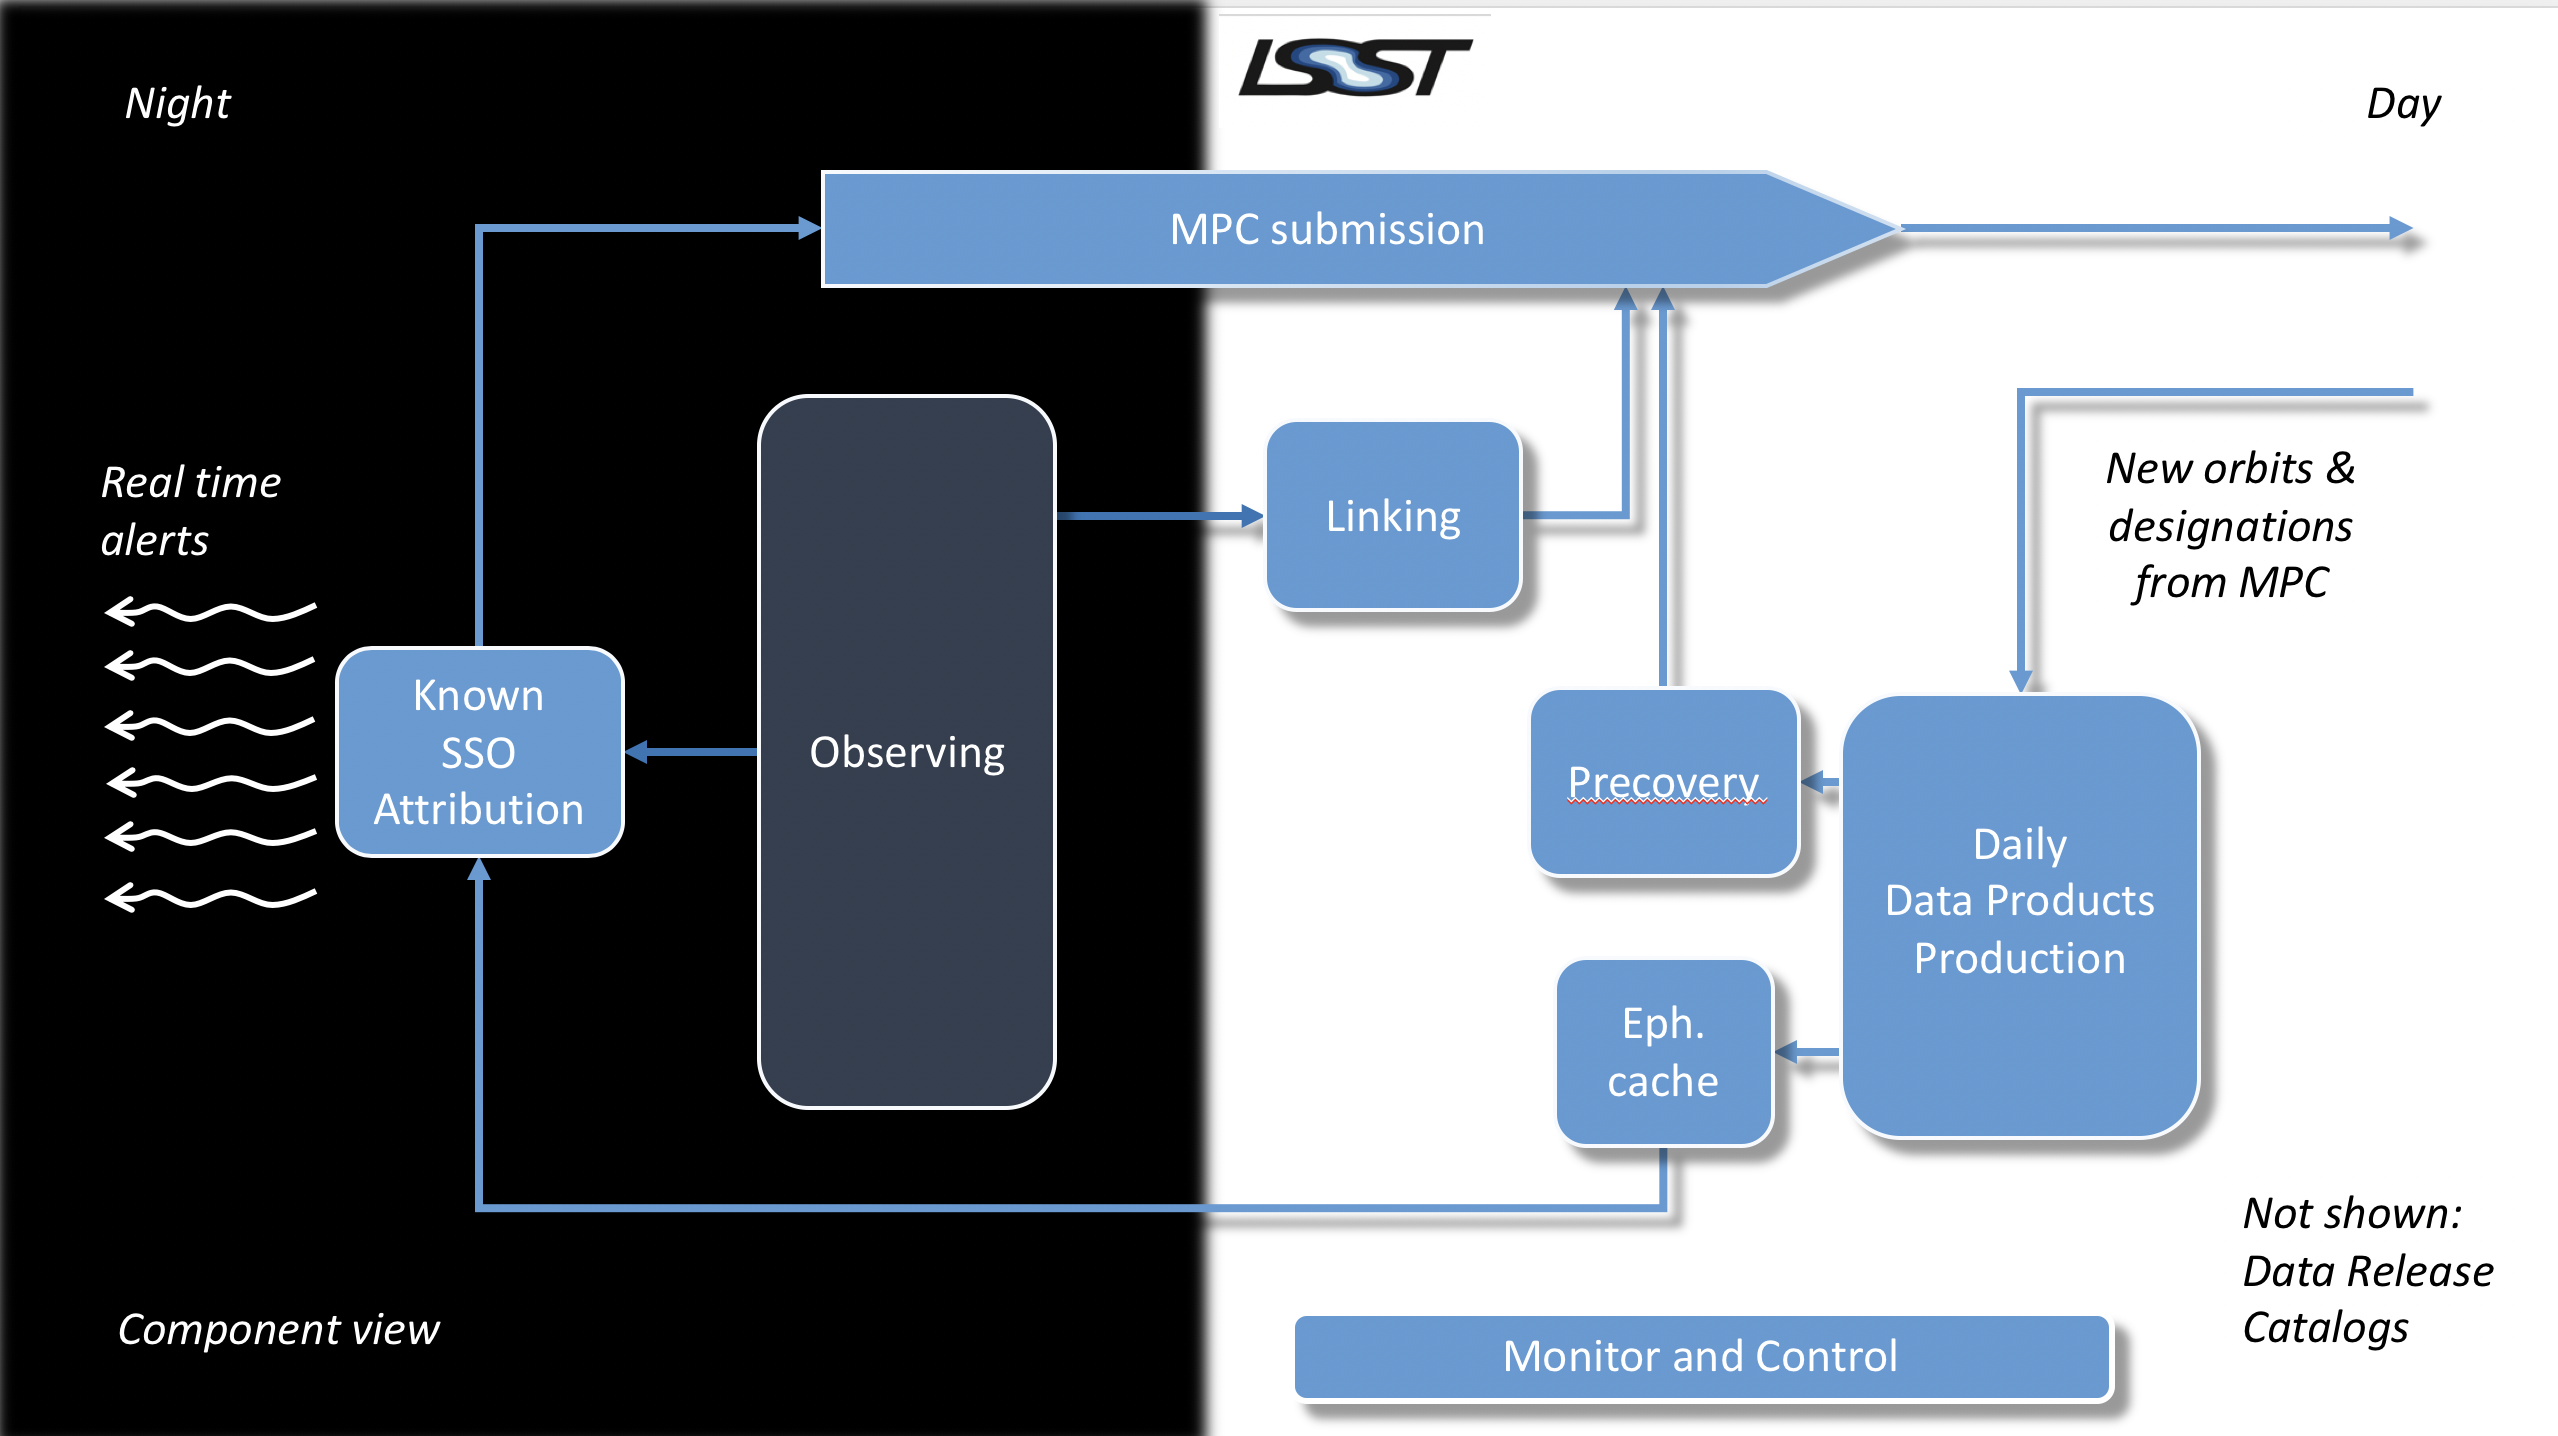
\includegraphics[scale=0.27]{./figs/mops2.png}
\end{center}
\caption{Concept of the \gls{LSST} Solar System Processing cycle.}
\label{fig:mops}       % Give a unique label
\end{figure}
%During operations the LSST will produce roughly 20TB of data per night. 
The \gls{LSST} is expected to discover millions of Solar System objects (SSOs) over the course of its ten years of operation \citep{jones2015asteroid}. 
Past assessments of discovery yields of future surveys see the \gls{LSST} becoming the dominant contributor of Solar System \gls{Object} (\gls{SSO}) related data to the \gls{IAU} Minor Planet \gls{Center} (\gls{MPC}) \citep{LSSTscibook2009}. The currently agreed upon strategy sees \gls{LSST} deliver astrometric and photometric observations of 
known SSOs as well as observations that represent potential discoveries after every night of operations.
Figure \ref{fig:mops} shows a corresponding schematic of the proposed \gls{LSST} \gls{SSO} processing \gls{pipeline}. 
Apart from Space Situational Awareness (\gls{SSA}) and planetary defense agencies that are mostly concerned with the capabilities of the \gls{LSST} to discover near-Earth asteroids, services that ingest and process \gls{LSST} data on a regular basis, such as the \gls{MPC}, 
have a great interest in estimates regarding the predicted data \gls{flux} directed their way. This requires accurate estimates regarding the actual number of predicted \gls{SSO} observations and discoveries. Early estimates stem from the \gls{LSST} Science Book \citep{LSSTscibook2009}. 
%\begin{table}
%\begin{center}
%\caption{Summary of small body populations observed with LSST as of 2015, from \citep{jones2015asteroid}.}
%\label{tab:table1}
% {\scriptsize
%  \begin{tabular}{|l|c|c|}
%  \hline\hline
%Population & known as of 2015 &  LSST discoveries$^1$ \\ \hline
%Near Earth Objects (NEOs) & 12,832 & 100,000   \\\hline
%Main Belt Asteroids (MBAs) & 636,499 & 5,500,000 \\ \hline
%Jupiter Trojans & 6,387 & 280,000  \\ \hline
%TransNeptunian and Scattered Disk Objects (TNOs and SDOs) & 1,921 & 40,000  \\ \hline\hline
% \end{tabular}
%  }
% \end{center}
%\vspace{1mm}
% \scriptsize{
% {\it Notes:}\\
%  $^1$)Expected at the end of LSST's ten years of operations.}
%\end{table}
As some progress has been made in this respect, both in scientific literature and in the \gls{LSST} project, it is the aim of this \gls{DMTN} to summarize and, where necessary, to provide updated \gls{LSST} \gls{SSO} observation and discovery rates as well as their uncertainties. This information is intended to inform internal and external services affected by \gls{SSO} discoveries.
The remainder of this \gls{DMTN} is structured as follows: Section \ref{sec:lsstss} briefly describes the \gls{LSST} survey and the simulation setup. Section \ref{sec:neo} provides a summary of previous work as well as a brief update on near-Earth asteroid discovery with the \gls{LSST}. Section \ref{sec:mba} discusses \gls{LSST} capabilities to discover Main Belt Asteroids that constitute the main source of \gls{LSST} \gls{SSO} observations. In section \ref{sec:delay} the impact of delayed \gls{LSST} operations and Solar System processing on discovery requirements is studied. Section \ref{sec:noise} assesses in how far unattributed \gls{SSO} observations could contribute noise to \gls{LSST} data. As MBA observations dominate \gls{SSO} observations section \ref{sec:data} discusses likely data rates that \gls{LSST} has to submit to the \gls{IAU} Minor Planet \gls{Center} (\gls{MPC}) on a nightly basis. Section \ref{sec:other}  looks at other \gls{SSO} populations and section \ref{sec:conclusions} concludes this report.

%According to the MPC, ingesting additional information on known objects can be performed with relatively little effort. 
%Confirming and providing preliminary orbits for potential discoveries, on the other hand, requires more resources.
%
%Updated predictions on how many SSOs LSST will discover 
%are, thus, of great interest, since they can serve as guideline for future infrastructure requirements. 
\section{LSST survey simulation} \label{sec:lsstss}
The proposed observation strategy for the \gls{LSST} survey used in this work is described in \href{http://astro-lsst-01.astro.washington.edu:8080/multiColor?runId=1#Fivesigmadepth}{baseline2018}. Its sky coverage, inter and intra-night gaps as well as the performance in terms of median and maximum five sigma depth is shown in Figure \ref{fig:gaps}. 

\begin{figure}[tb!]
\begin{tabular}{c}
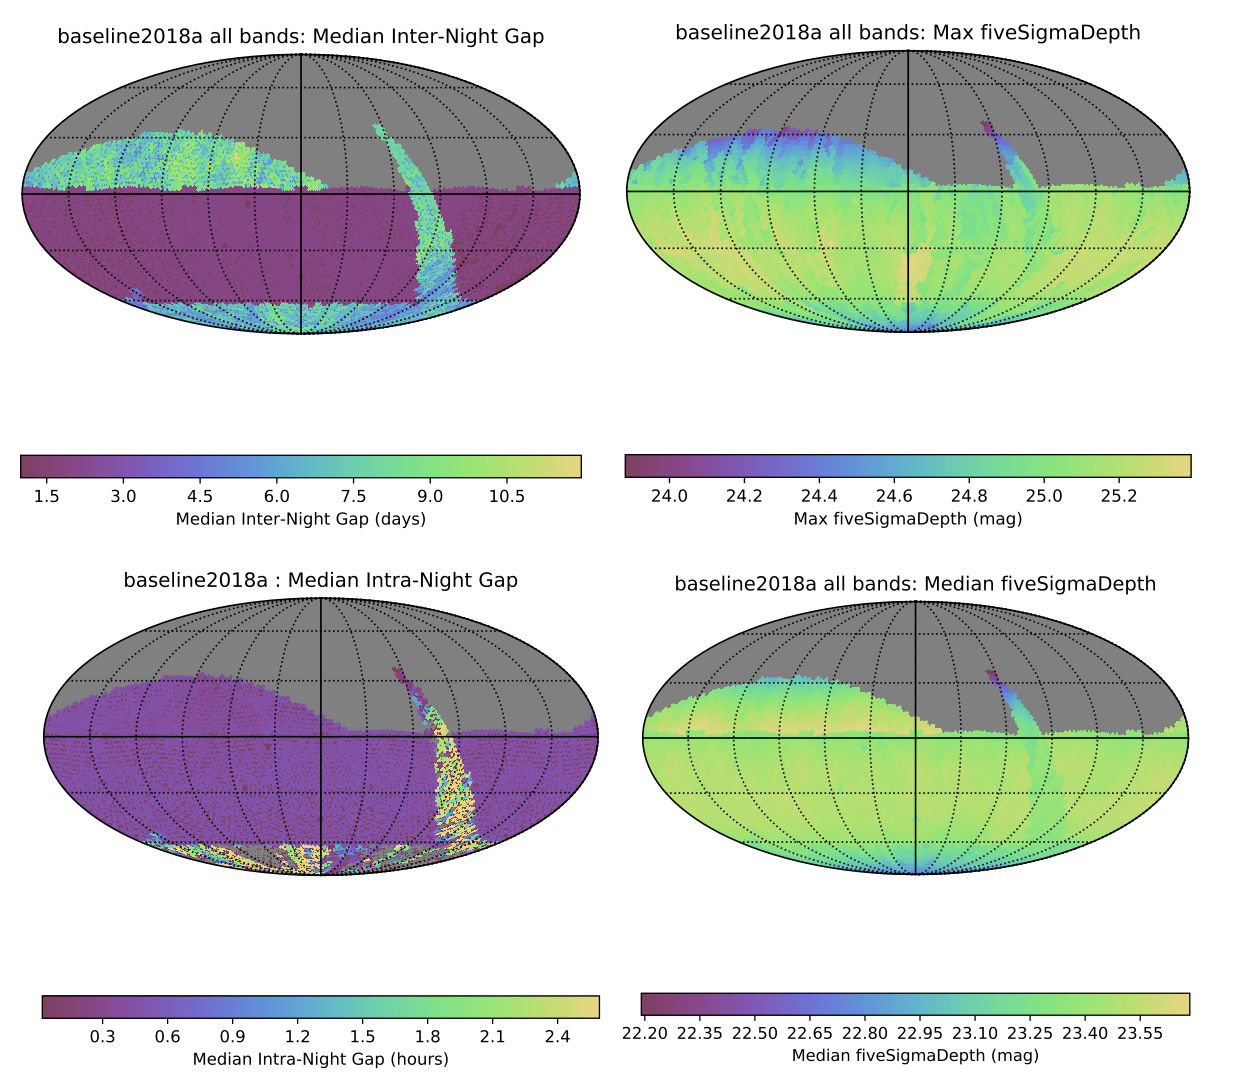
\includegraphics[width=1\linewidth]{figs/baseline2018a.png}
\end{tabular}
\caption{LSST survey simulation "baseline2018a". The left column shows Intra (top) and inter-night gaps (bottom) between returns to the same pointing. In the right column maximum (top) and median (bottom) five sigma depths are shown.}
\label{fig:gaps}       % Give a unique label
\end{figure}
%
During the \gls{Wide-Fast-Deep} (WDF) survey \gls{LSST} is expected to reach median five signal depths around 23.5mag with median inter and intra-night gaps of 1.5 days and 20 mins, respectively. Such a cadence facilitates the construction of nightly tracklets, successive observations of
moving objects spanning a short arc. Tracklets of individual objects can then be linked over several nights resulting in the discovery of SSOs.
Two types of survey simulation software frameworks were used to generate and validate \gls{LSST} \gls{SSO} discovery statistics, namely
\begin{itemize}
\item \href{https://epyc.astro.washington.edu/~lynnej/sims_movingObjects/lsst.sims.movingObjects.html}{LSST Sims\_movingObjects (SIMS\_MO)}
\item \href{https://github.com/eggls6/openobs}{Open Observation Simulator (OPENOBS)}
\end{itemize}
The former is a high fidelity simulator that includes N-body numerical orbit propagation, the actual \gls{LSST} \gls{camera} model, as well as color information of asteroids. SIMS\_MO is capable of performing accurate observation simulations for up to several 100k of SSOs. Although that constitutes only a fraction of the true MBA population, information on expected survey completeness statistics can be extracted through sampling of individual orbits over a grid of absolute magnitudes. 
OPENOBS is capable of performing survey simulations on the entire expected MBA population (around 100M objects) albeit with a lower fidelity. Instead of N-body propagation unperturbed heliocentric Keplerian orbits of SSOs are assumed. The \gls{LSST} \gls{camera} \gls{footprint} is simulated, but the exact geometry including chip gaps has not been taken into account in OPENOBS simulations. Instead, the fill factor of the \gls{camera} system as calculated in \citet{veres2017high} was used to statistically filter observations. Spectral energy distributions (SEDs) of asteroids are assumed to be flat in OPENOBS simulations, while S- and C-type asteroid \gls{SED}s are used in SIMS\_MO (Figure \ref{fig:sed}). The magnitude cutoff in our simulation was chosen to be H=25 mag corresponding to MBA diameters between 19m-60m depending on object albedo (0.5-0.05).
\begin{figure}[tb!]
\begin{center}
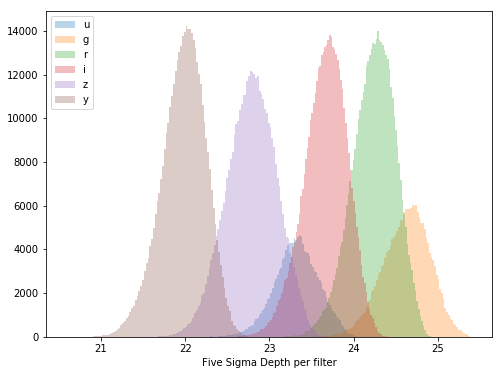
\includegraphics[width=0.5\textwidth]{figs/5sig_filter.png}\\
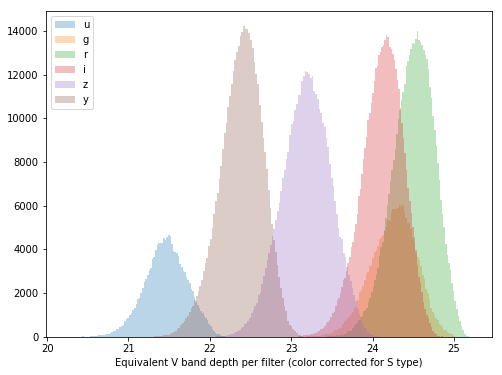
\includegraphics[width=0.5\textwidth]{figs/5sig_filter_S.png}\\
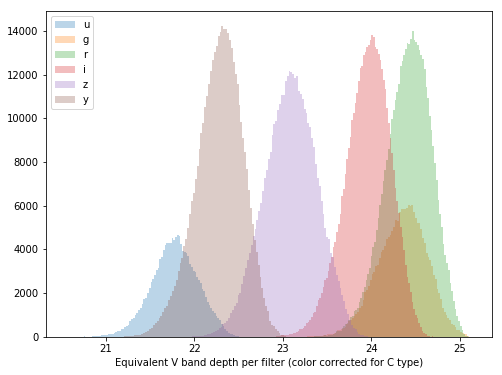
\includegraphics[width=0.5\textwidth]{figs/5sig_filter_C.png}
\end{center}
\caption{A comparison of \gls{LSST} depths per filter for a flat \gls{SED} (top), an \gls{SED} corrected for S-type asteroids (center) and C-type asteroids (bottom), respectively.}
\label{fig:sed}       % Give a unique label
\end{figure}
%Combining results from SSO population studies and LSST's expected performance we suggest that the  
%MBAs will dominate SSO discoveries.
%
%800k Mag < H
% 
% trailing losses
% probabilistic 50\% 
% default uses fading
% vignetting
% camera orientation is includeded
\clearpage
\section{Near-Earth Asteroids}\label{sec:neo}
Substantial efforts have been undertaken to assess the potential of the \gls{LSST} of discovering near-Earth asteroids \citep[e.g.][]{ivezic2006lsst,jones2015asteroid,grav2016modeling,veres2017near,veres2017high,jones2018large,ivezic2019lsst}. The current consensus is that \gls{LSST} is capable of achieving around 60\% integral completeness NEOs with absolute magnitude brighter than 22, roughly 140m in size and larger. Together with other existing \gls{NEO} surveys that number can be increased to 73\% with the current \gls{LSST} survey strategy. The prospects for discovering Potentially Hazardous Asteroids (PHAs) are even better, with a predicted 81\% completeness at the end of the nominal \gls{LSST} survey \citep{ivezic2019lsst}. The completeness fraction is largely independent of \gls{NEO} population models such as \citep[S3M,][]{s3m} and \citet{granvik2018neos}, see Figure \ref{fig:neo_compl}. In contrast, the actual number of discovered objects varies considerably as shown in Figure \ref{fig:neo_count}. \gls{LSST} discoveries for asteroids brighter than H=25mags range from 50k to 100k over the 10yrs of the \gls{LSST} survey, which corresponds to 2.5 to 5 times the number of currently known NEOs (Figure \ref{fig:neo_current}).
Uncertainties in the \gls{NEO} population model are the most significant contributors to the uncertainty in the number of \gls{NEO} discoveries. All \gls{NEO} simulations have been performed with SIMS\_MO.
\begin{figure}[tb!]
\begin{center}
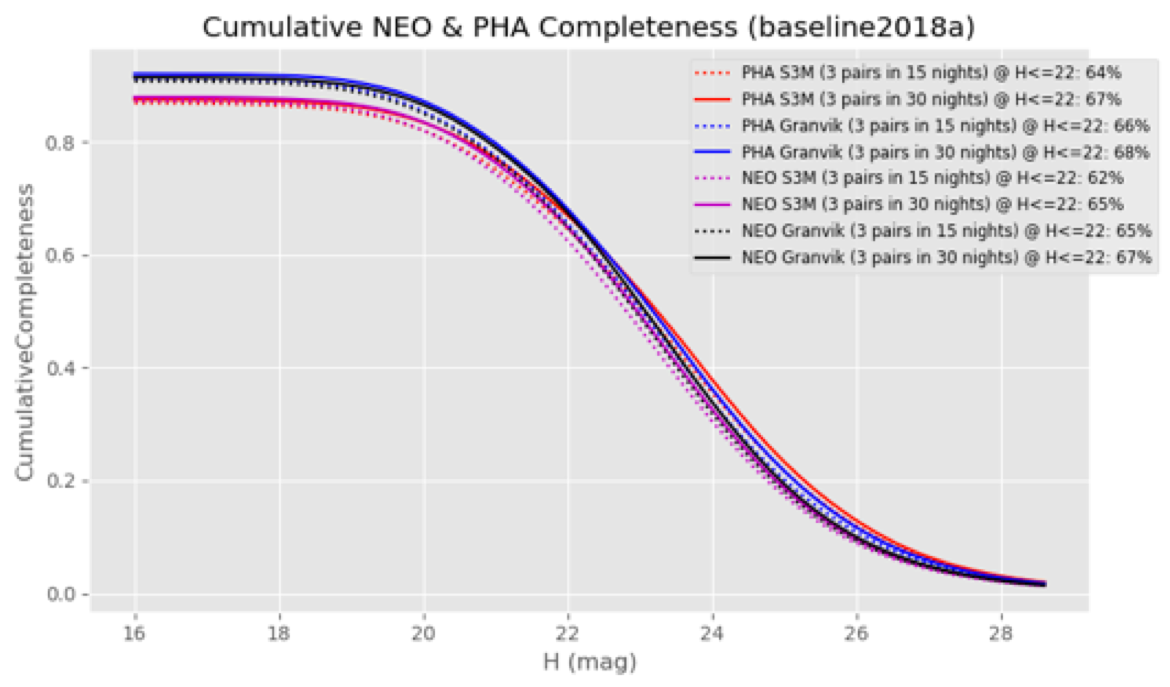
\includegraphics[width=0.65\linewidth]{figs/neo2.png}
\end{center}
\caption{Cumulative near-Earth asteroid (NEA) and Potentially Hazardous Asteroid (\gls{PHA}) completeness at the end of the 10yr \gls{LSST} survey for different asteroid population models \citep[S3M,][]{s3m} and \citet{granvik2018neos}. Results for three pairs of observations over 15 nights are compared to similar detection conditions over 30 nights.}
\label{fig:neo_compl}       % Give a unique label
\end{figure}

\begin{figure}[tb!]
\begin{center}
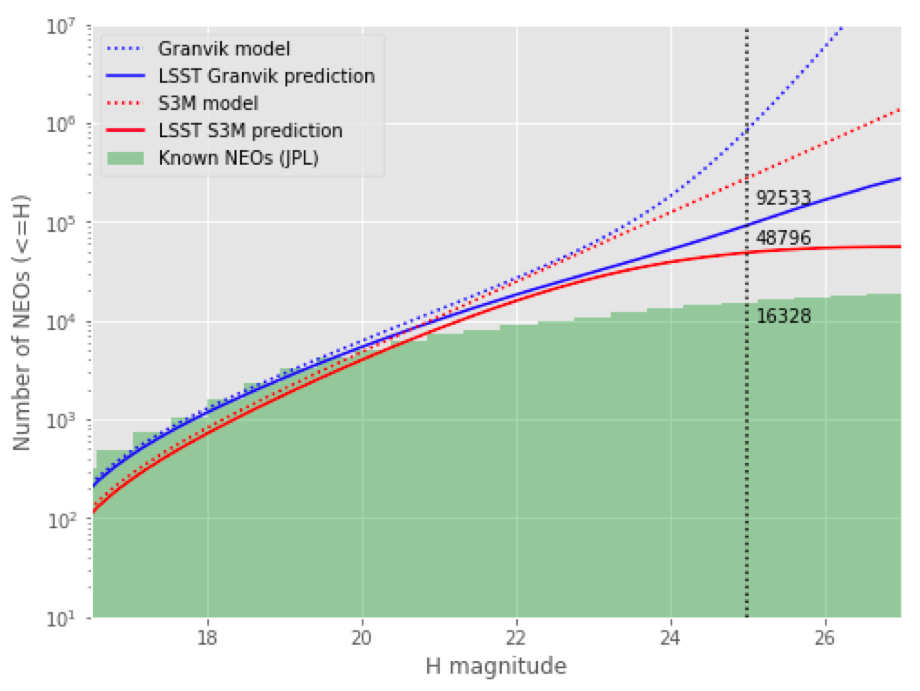
\includegraphics[width=0.65\linewidth]{figs/neo1.png}
\end{center}
\caption{Number of NEOs discovered with the \gls{LSST} for different population models \citep[S3M,][]{s3m} and \citet{granvik2018neos}. 
The prediction curves represent the cumulative number of discovered NEOs as a function of their absolute magnitude H, while the model curves show the number of expected objects in the population.}
\label{fig:neo_count}       % Give a unique label
\end{figure}

\begin{figure}[tb!]
\begin{center}
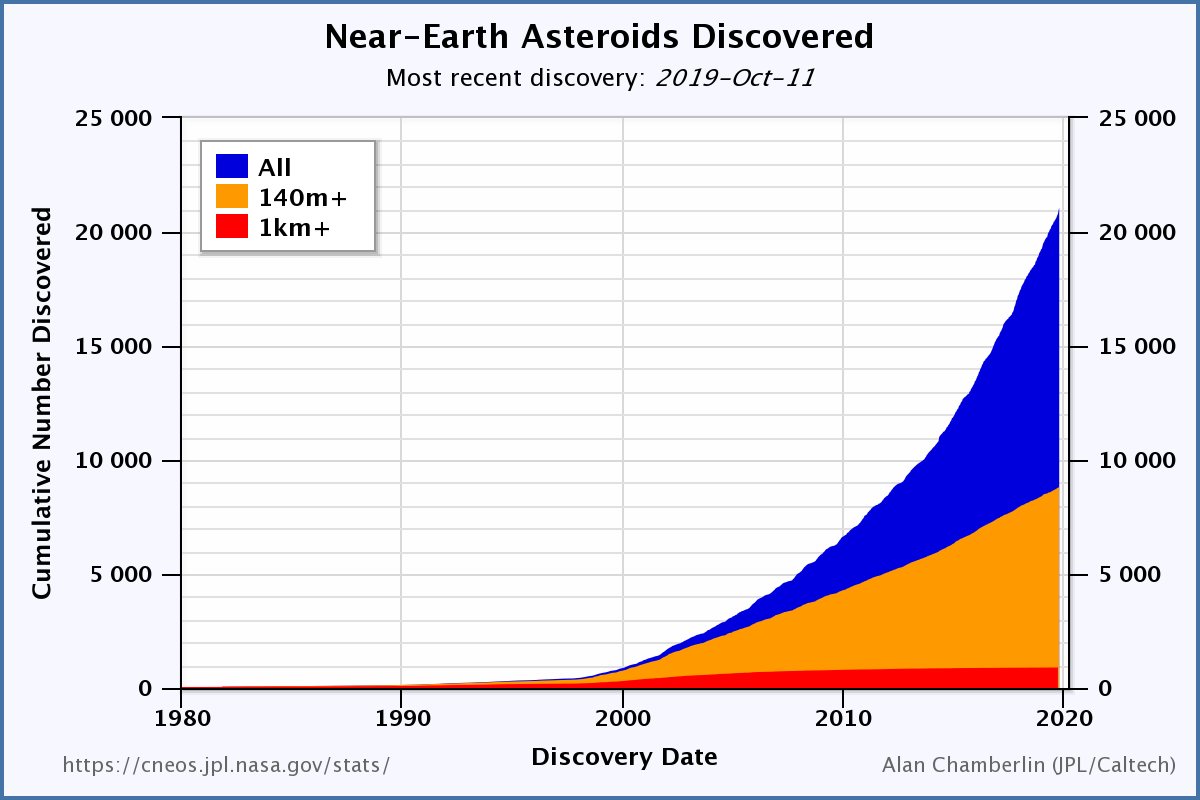
\includegraphics[width=0.65\linewidth]{figs/nea_vs_time_chart.png}
\end{center}
\caption{Number of known NEOs as a function of time. \gls{Source}: \gls{NASA} \gls{JPL}/Caltech}
\label{fig:neo_current}       % Give a unique label
\end{figure}

\clearpage

\section{Main Belt Asteroids} \label{sec:mba}
The vast majority of SSOs accessible to the \gls{LSST} populate the Main-Belt (\gls{MB}) between Mars and Jupiter \citep{LSSTscibook2009}. Estimates on \gls{SSO} discovery and observation statistics presented in this document are, therefore, be based on simulations of Main-Belt asteroid (MBA) observations with the \gls{LSST}. 
In order to quantify the number of potential \gls{LSST} discoveries, we adopt a simple model for the size-frequency and orbit distribution of MBAs of the form
\begin{equation}
 N(H)=\beta\;10^{\;\alpha H}
 \label{eq:lsw}
\end{equation}
where $N$ is the number of MBAs, $H$ the absolute magnitude, and $\alpha$ and $\beta$ determine the slope and the anchor value of the log-linear fit, respectively.
The parameters in equation (\ref{eq:lsw}) were derived from the current MBA population using actual data of the main belt supplied by the \gls{MPC}. 
Assuming the bight main belt population is essentially complete up to $H=14.5$mag, we can fit lower and upper bounds on the size-frequency distribution that we extrapolate to fainter objects. The corresponding results are presented in Figure \ref{fig:mba_pop} as well as in Table \ref{tab:mbapop}.
In order to guarantee that the slope and anchor parameters for the MBA population are not influenced by the specific choice of the bin-size in $H$ we derived the underlying distribution $n(H)$ using kernel density estimation where
\begin{equation}
 n\;(H)=\frac{1}{I\,b} \sum_{i=1}^{I} K\left(\frac{H-H_i}{b}\right),
 \label{eggl:eq:kernel}
\end{equation}
where $K$ is the (Gaussian) kernel and $b$ a smoothing parameter, respectively. The resulting slopes are compatible with \citet{jedicke2002} who find local slopes between $0.24<\alpha<0.58$ for MBAs with $H>10$, as well as with size-frequency distributions from Trans-Neptunian Objects (TNOs), where $\alpha\approx0.66$ \citep{bernstein2004}.
Orbital elements of synthetic MBAs are sampled from the joint distribution of orbital elements of the current main belt. We assume that the size-frequency and orbital element distribution are essentially uncorrelated. While, strictly speaking, this is not the case for asteroids that belong to families, a similar approach was used to create the S3M \citep{s3m}, a synthetic Solar System model for \gls{Pan-STARRS}.
In contrast to the "bracketing" approach adopted in this work via estimating upper and lower bounds to the size-frequency distribution in the main belt, the MBA population in the S3M is based on work by \citet{jedicke2002}. A comparison between the here adopted model and \citet{jedicke2002} used in S3M can be seen in Figure \ref{fig:mba_pop}.
\begin{table}[t!]
\begin{center}
\begin{tabular}{cllr}
\hline
model & $\alpha$ & $\beta$ & $N_{tot}(H \le 25)$ \\
\hline
A & 0.3 &  2.29 & 104 $\times 10^{6}$ \\
B & 0.56 &4.43 $\times 10^{-4}$ & 34.5$\times 10^{9}$\\
\hline
\end{tabular}
\end{center}
\caption{Main Belt Asteroid (MBA) population models used in this work. The parameters $\alpha$ and $\beta$ are input to equation (\ref{eq:lsw}). $N_{tot}$ is the estimate for the total asteroid population with $H\le 25$ mag. }
\label{tab:mbapop}
\end{table}
%%%
\begin{figure}[b!]
%\includegraphics[scale=.65]{pics/ptype_gf_a1.png}
\begin{center}
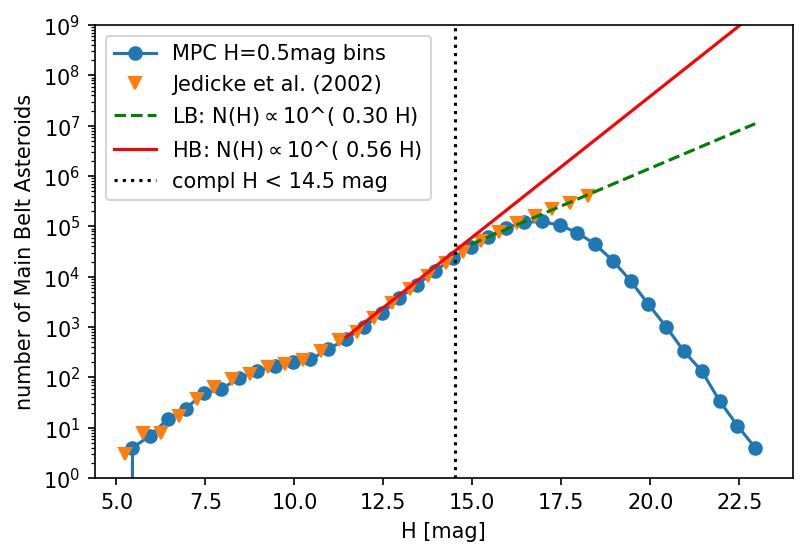
\includegraphics[scale=.8]{figs/mpc_population_4.png}
\end{center}
\caption{MBA population extrapolation using a continuous (red, green) and broken $H(N)$ power law (orange), respectively.}
\label{fig:mba_pop}       % Give a unique label
\end{figure} 
%
The current strategy of the \gls{LSST} Solar System Processing is to send only those observations of SSOs to the \gls{MPC} that have a high likelihood of being either associated to know objects or new discoveries. 
In order to minimize false positives in potential asteroid discoveries, observations of new objects are only submitted, if they are detected least twice per night on three distinct nights (so-called "three nighters"). The three nights do not have to be consecutive. Detections can be spread over a window of 15-30 nights. Assuming a linking efficiency close to 100\%, such "three-nighters" can be turned into preliminary orbits that have a high likelihood of belonging to newly discovered objects. 
The expected completeness as a function of absolute magnitude (a proxy for the size of objects) for MBAs is shown in Figure \ref{fig:mba_compl} after 6 months, 1 year, 2 years and after 10 years of \gls{LSST} operations.
\begin{figure}[b!]
%\includegraphics[scale=.65]{pics/ptype_gf_a1.png}
\begin{center}
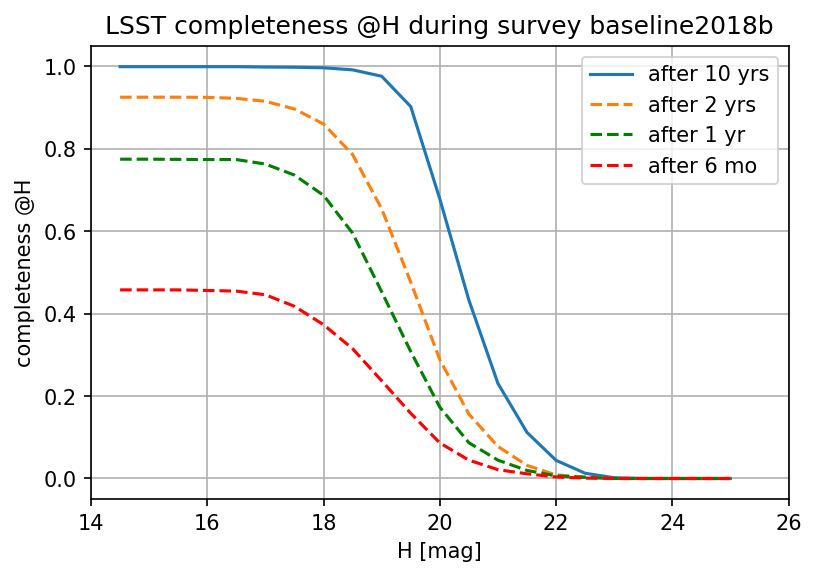
\includegraphics[scale=0.7]{figs/mba_completeness3.png}
\end{center}
\caption{Survey completeness for MBAs at a given absolute magnitude (H) as a function of time.}
\label{fig:mba_compl}       % Give a unique label
\end{figure}
%
The graph shows that after two years of survey more than 90\% of kilometer sized MBAs will have been discovered.
By the nominal end of the \gls{LSST} survey we know essentially all MBAs with diameters of half a kilometer and larger.
The total number of discovered MBAs as a function of absolute magnitude in presented in Figure \ref{fig:mba_disc}. Results for the two  size-frequency distributions probed are 
shown for both software packages, SIMS\_MO and OPENOBS. Formal errors for SIMS\_MO discoveries are based on the sample size selected from the assumed size frequency distribution.  
A comparison of Figures \ref{fig:mba_compl} and \ref{fig:mba_disc} shows that results for SIMS\_MO and OPENOBS are very similar where \gls{LSST} is expected to be essentially complete (H$\approx19$ mag). For smaller and fainter objects discovery rates differ slightly leading to a discrepancy of roughly 10\%, which is negligible compared to the uncertainties in the expected number of MBAs. 
%
\begin{figure}[tb!]
\begin{center}
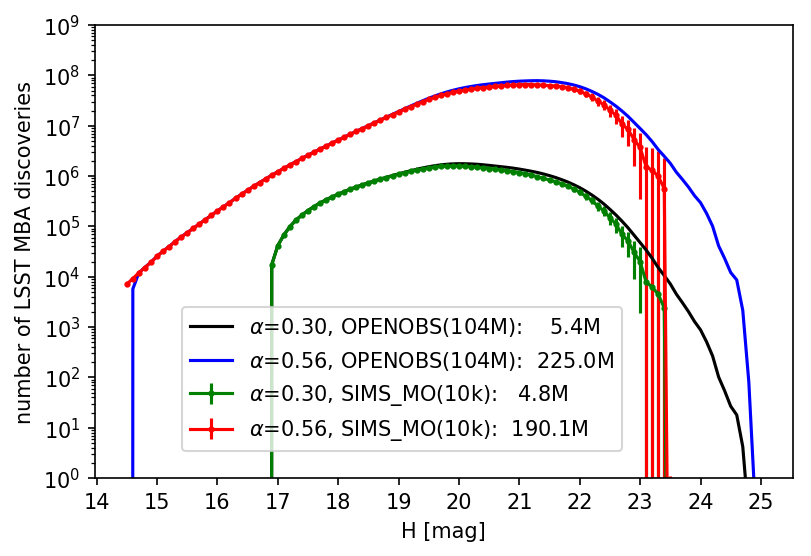
\includegraphics[scale=0.9]{figs/mba_disc3.png}
\end{center}
\caption{LSST Main Belt asteroid discoveries as a function of absolute magnitude for two different size-frequency distributions (population model A and \gls{B}) and simulation software packages OPENOBS and SIMS\_MO. See text for details.}
\label{fig:mba_disc}       % Give a unique label
\end{figure}
%
Figure \ref{fig:mba_disc_stats} shows the expected number of \gls{LSST} MBA discoveries per night as predicted by OPENOBS simulations. The number of discovered objects ranges from a few per night to 100 000 discoveries depending on the momentary cadence and ecliptic latitude. Figure \ref{fig:mba_disc_stats} provides statistical information on how many nights are expected to yield a certain number of discoveries. The conservative size-frequency distribution sees an average of 2000 discoveries per night\footnote{not observed night} during the ten year survey for more than 200 nights. Nights with more objects are rare but do occur. Discovery maxima of roughly 100 000 discoveries per night can occur. A steeper size-frequency distribution of MBAs (population model \gls{B}) would see nights with more than 10 million discoveries. 

Figure \ref{fig:mba_disc_yr} shows the number of expected MBA discoveries for each of the ten years of \gls{LSST} operations. If Solar System Processing (\gls{SSP}) stars right away, the majority of objects will be discovered during the first years of the \gls{LSST} survey. Figures \ref{fig:mba_compl} and \ref{fig:mba_disc_yr} demonstrate the power of the \gls{LSST} to quickly distinguish between various hypothesis on the size-frequency distribution in the main belt. 
%
\begin{figure}[tb!]
\begin{center}
\begin{tabular}{cc}
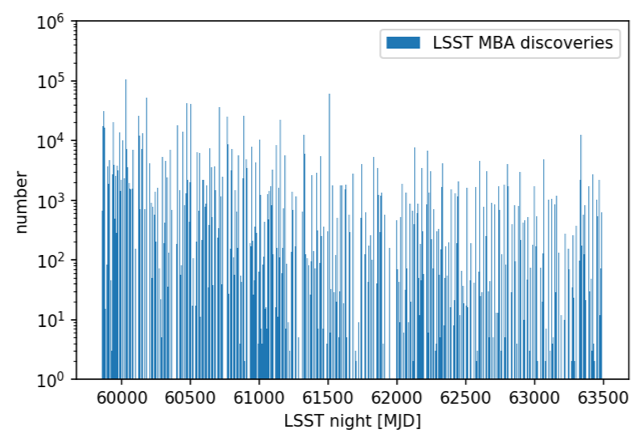
\includegraphics[width=0.5\linewidth]{figs/disc_per_night.png} &
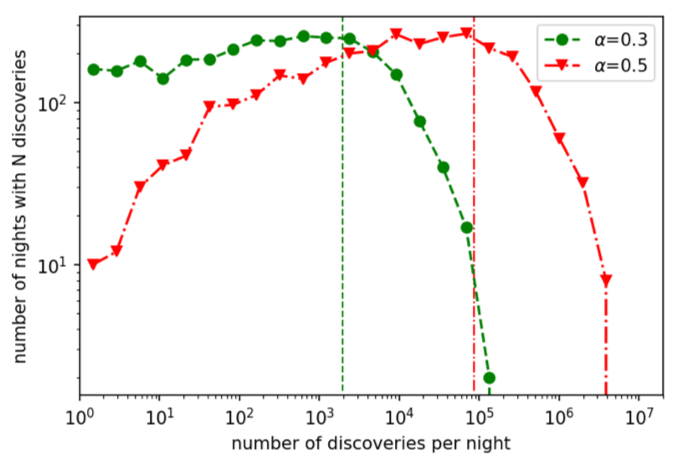
\includegraphics[width=0.50\linewidth]{figs/disc_stat.png}
\end{tabular}
\end{center}
\caption{Left: \gls{LSST} Main Belt Asteroid (MBA) discoveries per observed night for population model A. Right: Number of nights with a certain discovery yield versus number of discoveries per night for two different MBA size-frequency distributions.}
\label{fig:mba_disc_stats}       % Give a unique label
\end{figure}

\begin{figure}[tb!]
\begin{center}
\begin{tabular}{cc}
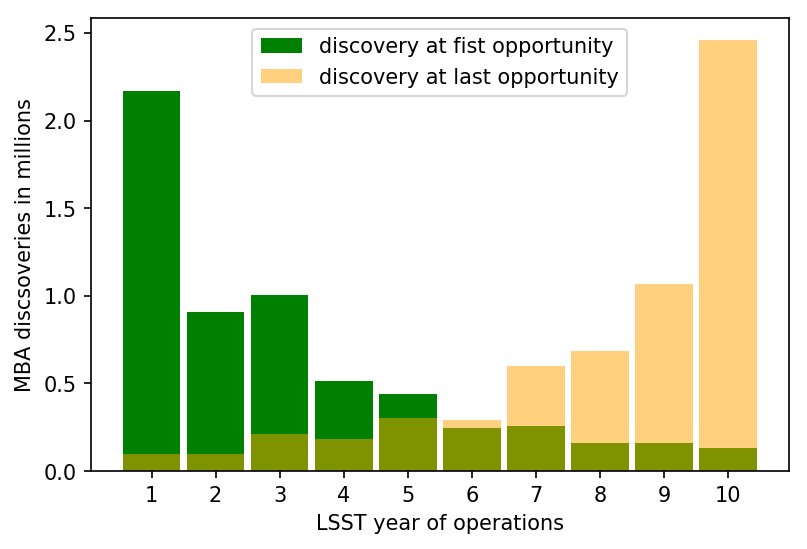
\includegraphics[width=0.5\linewidth]{figs/discovery_time.png} &
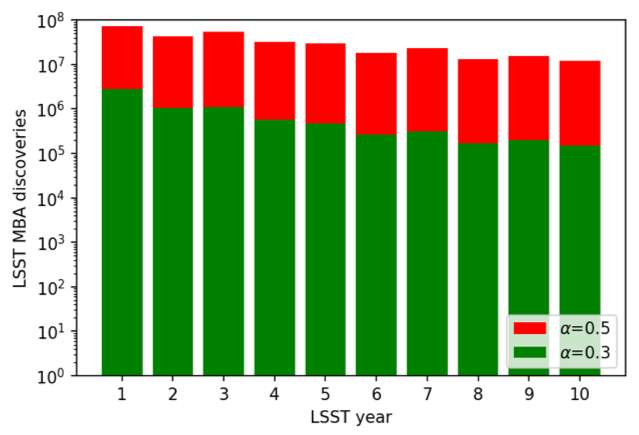
\includegraphics[width=0.5\linewidth]{figs/disc_per_yr2.png}
\end{tabular}
\end{center}
\caption{LSST Main Belt Asteroid (MBA) discoveries per year on a linear (left) and logarithmic scale (right) assuming 100\% linking efficiency. The left panel compares yields for early and late discovery scenarios. The right panel shows discovery yields for population models A (green) and \gls{B} (red) in an early discovery scenario.}
\label{fig:mba_disc_yr}       % Give a unique label
\end{figure}
%
The on-sky distribution of observations of discoverable MBAs is shown in Figure \ref{fig:mba_obs_sky}. The darker spots showing an increased number of observations per square degree correspond to the \gls{LSST} deep drilling fields from small to high Right Ascension values: ELAIS S1, \gls{XMM}-LSS, Extended Chandra, Deep Field-South and COSMOS.
\begin{figure}
\begin{center}
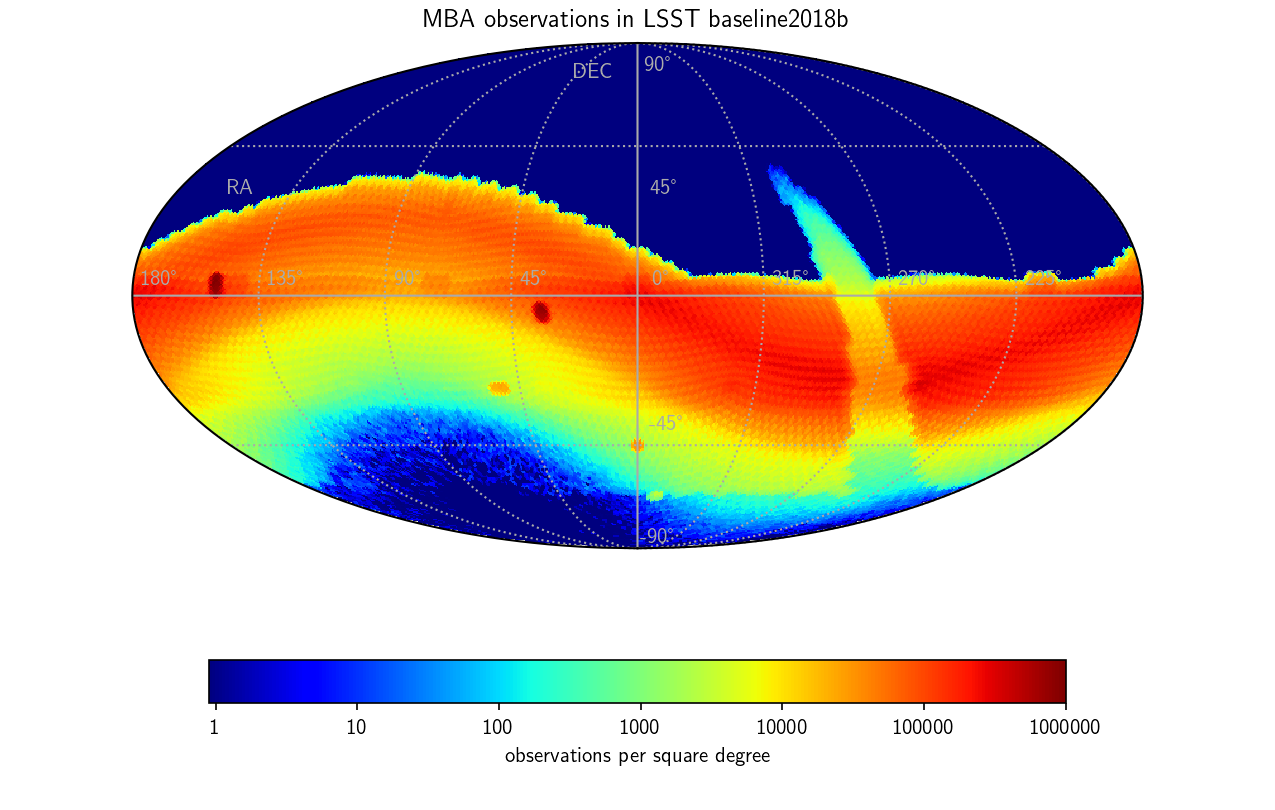
\includegraphics[width=0.70\linewidth]{figs/mba_obs_hpmap.png}
\end{center}
\caption{On-sky (ICRF) distribution of observations per square degree of MBAs (population model A, 14.5 $\le$ H [mag] $\le$ 25) discoverable with the \gls{LSST}.The dark spots correspond to the \gls{LSST} deep drilling fields from right to left: ELAIS S1, \gls{XMM}-LSS, Extended Chandra, Deep Field-South and COSMOS.}
\label{fig:mba_obs_sky}       % Give a unique label
\end{figure}
%
Many asteroids are observed frequently enough so that they can be discovered later on, if initial discovery opportunities were missed (Figure \ref{fig:do}). Missed discovery opportunities may result from a failure to identify and/or link possible tracklets in the Solar System Processing \gls{pipeline}, or a hardware/software malfunction in the telescope itself, for instance. Bright objects have on average 200 discovery opportunities. This number drops fast for fainter objects, however. Discovery opportunities for MBAs generally reoccur after a synodic period between the Earth and the Main belt ($\approx 500$days) as can be seen from Figure \ref{fig:do}. Most of the very faint objects have one discovery opportunity only. They populate the main diagonal in the right panel of Figure \ref{fig:do}. 
%
\begin{figure}[tb!]
\begin{tabular}{ll}
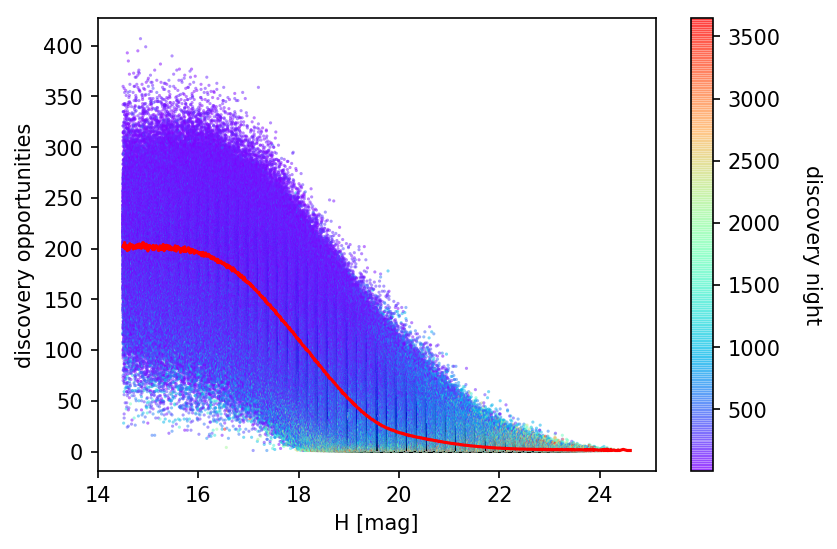
\includegraphics[width=0.5\linewidth]{figs/disc_opport3.png}
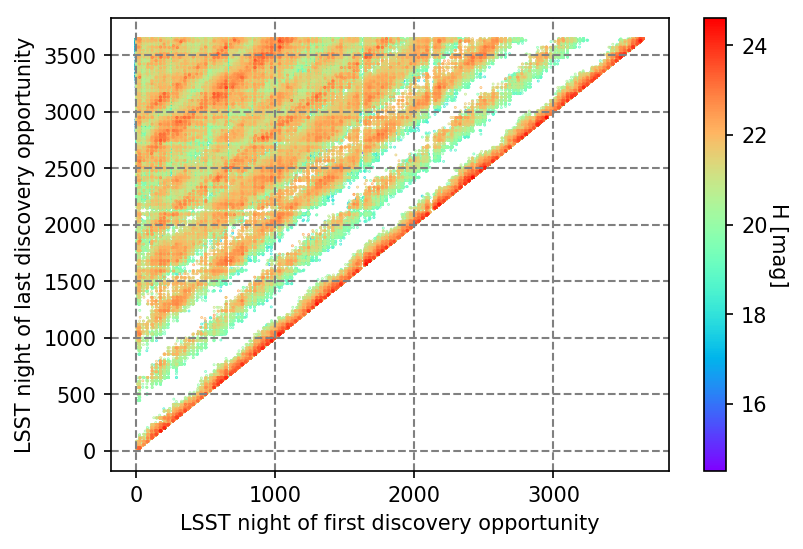
\includegraphics[width=0.5\linewidth]{figs/first_vs_last.png} &
\end{tabular}
\caption{Left: Discovery opportunities for MBAs as a function of their absolute magnitude (H). The red line indicates the median for each H bin. Right: First vs. last discovery opportunity for MBAs. The color coding indicates the \gls{LSST} night in which the object could be first discovered.}
\label{fig:do}       % Give a unique label
\end{figure}
\clearpage
%%%%%%%%%%%%%%%%%%%
\section{Impact of delayed \gls{LSST} operations and Solar System Processing} \label{sec:delay}
\begin{figure}[tb!]
\begin{center}
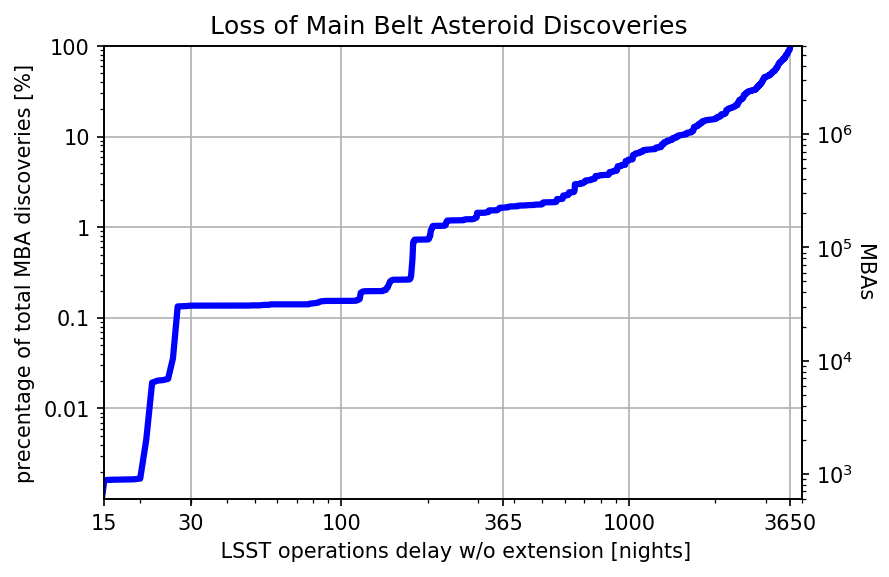
\includegraphics[width=0.70\linewidth]{figs/lost4.png}
\end{center}
\caption{Losses in MBA discoveries due to delayed operations of the \gls{LSST} (assuming no extension) for population model A.}
\label{fig:lost}       % Give a unique label
\end{figure}
Even in a worst case scenario where \gls{LSST} operations are significantly delayed, the majority of asteroids could still be discovered during the last years of the nominal period of operations (Figures \ref{fig:mba_disc_yr} and \ref{fig:lost}).\footnote{Note, that this is not necessarily true for near-Earth asteroids, since their discovery function is not as simple a function of the synodic period as it is for MBAs.} 
A delay in \gls{LSST} operations for a month would result in roughly 0.1\% of asteroids lost. Shortening operations for a 
a year would result in the loss of 2\% of main belt asteroid discoveries, roughly 200k objects.
A delay in Solar System Processing alone would have less dramatic consequences, if \gls{LSST} operations proceed nominally and data of SSOs is still collected.
The computational resources to reprocess the collected data do have to be accounted for, however. As can be gathered from Figure \ref{fig:rep}, an \gls{SSP} delay of a month requires the reprocessing of almost half a million objects with 20 million attributable observations. If \gls{SSP} were to be delayed for a year, for instance, in order to have high quality templates available, around two million objects with 100 million observations would need to be processed on top of the daily data releases. Although this constitutes a non-negligible computational effort, the planned, yearly \gls{LSST} data releases would be of similar magnitude. Hence, we do not anticipate a change in the computational requirements at this point, even if the \gls{SSP} were to be delayed.
That being said, timely Solar System Processing offers numerous advantages:
\begin{itemize}
\item The success of follow up observations hinges on a timely identification and publication of objects of interest.
\item A continuous rather than a blocked reduction of \gls{LSST} \gls{SSO} data can help avoid computational bottlenecks later in the survey.
\item Identifying detections belonging to SSOs can help decrease the number of ``false alerts".
\end{itemize}
A quantitative assessment of the latter point is presented in the next section.
%
\begin{figure}[tb!]
\begin{center}
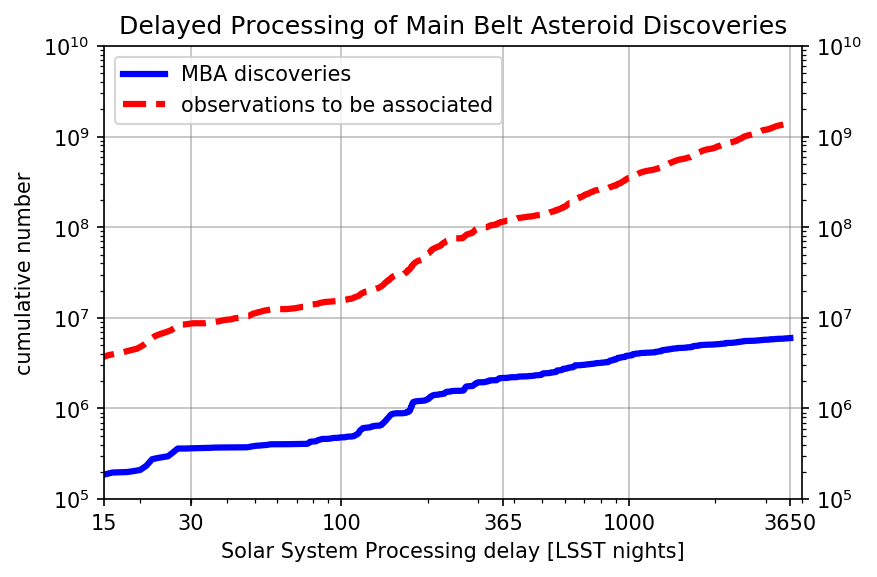
\includegraphics[width=0.70\linewidth]{figs/reprocessing4.png}
\caption{Cumulative number of MBAs (blue) and observations (red) that require reprocessing if \gls{SSP} is delayed. }
\end{center}
\label{fig:rep}       % Give a unique label
\end{figure}

\clearpage

\section{Solar System Objects as a \gls{Source} of Noise} \label{sec:noise}
\begin{figure}[tb!]
\begin{center}
\begin{tabular}{cc}
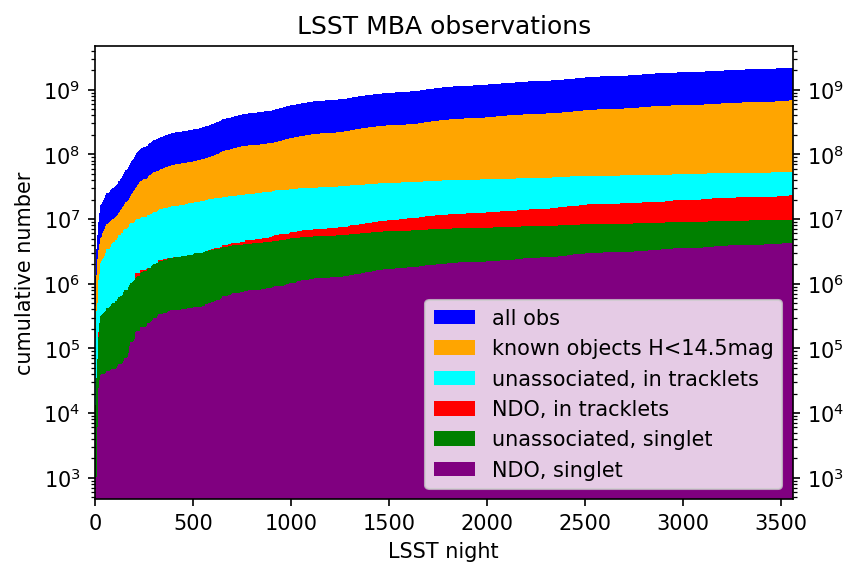
\includegraphics[width=0.5\linewidth]{figs/cum_un_obs_first.png} &
%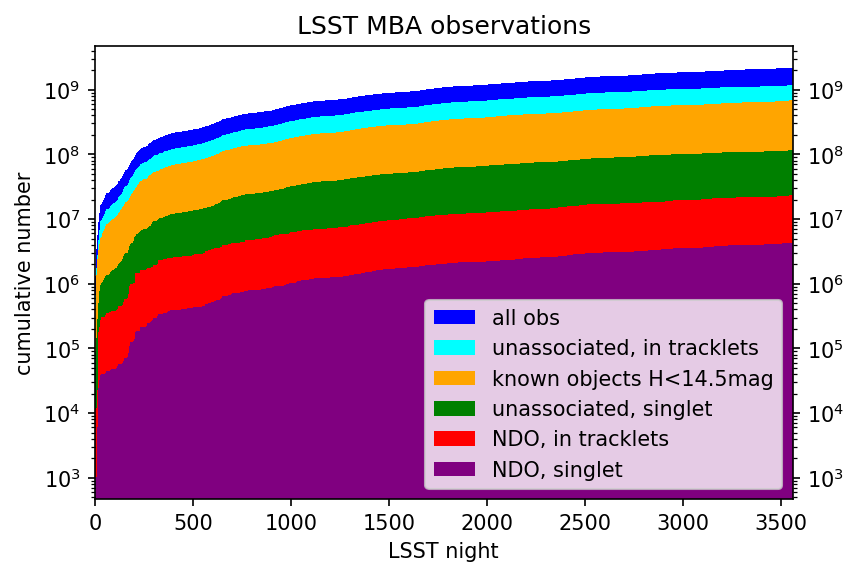
\includegraphics[width=0.45\linewidth]{figs/cum_un_obs_last.png}\\
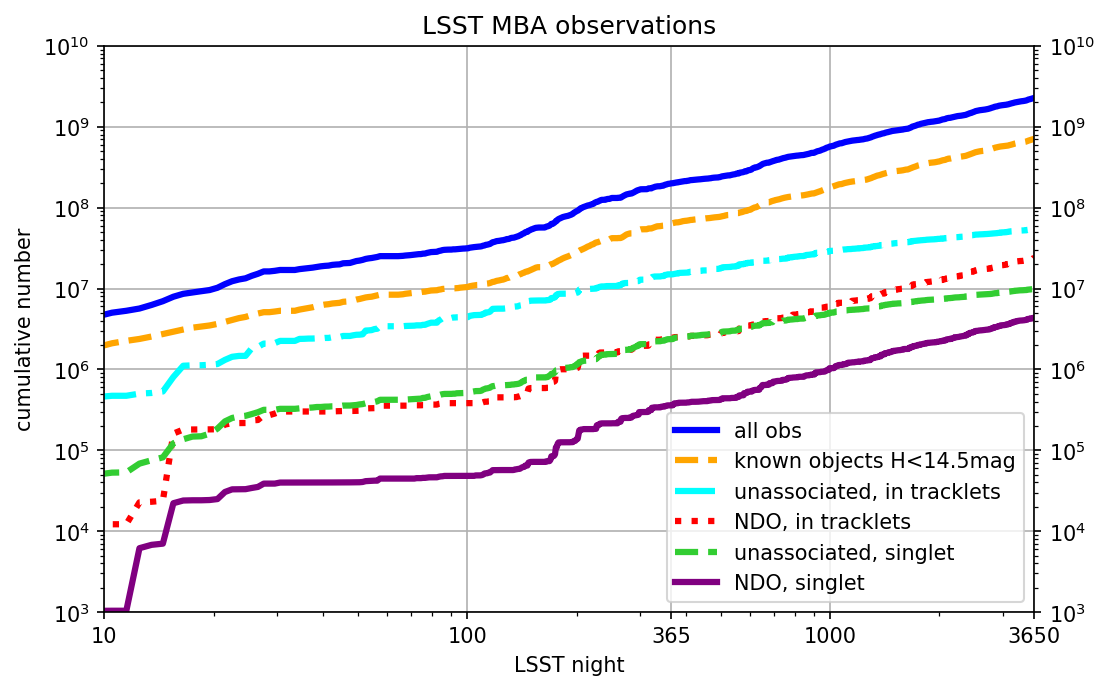
\includegraphics[width=0.5\linewidth]{figs/cum_un_obs_first2.png}\\
%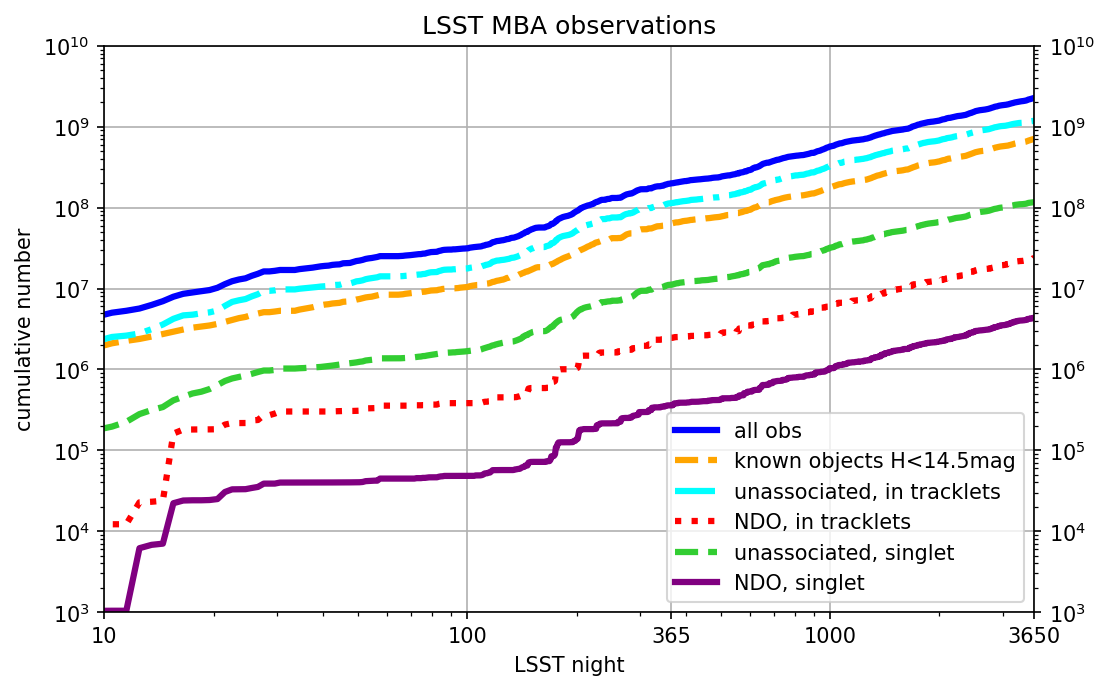
\includegraphics[width=0.45\linewidth]{figs/cum_un_obs_last2.png}\\
\end{tabular}
\end{center}
\caption{Cumulative number of \gls{LSST} observations of MBAs over time. The left panels shows all \gls{LSST} observations (blue), observations of bright, already known objects (orange), unassociated observations in tracklets (cyan) and singlets (green) and non-discoverable objects in trackelts (red) and singlets (purple). 
%The right panels display the corresponding curves for the case where all asteroids are discovered at the last instead of the first opportunity. 
The left panel is log linear, while the right panel contains a log-log plot. The corresponding numbers are presented in Table \ref{tab:mbaobs}.\label{fig:cum_un_obs}}
       % Give a unique label
\end{figure}
%
Not all new SSOs detected by the \gls{LSST} accumulate enough observations to count as ``discovered". 
The current discovery policy for SSOs requires repeated recurrence (three-nighters).  
An object must have at least two observations per night over three nights in a 15-30 night window to be considered a candidate object that can be sent to and validated by the \gls{MPC}.
Detections that can neither be linked to known objects nor grouped to form a new discovery are bound to contribute to the overall "noise" that may trigger false alerts, for instance. In order to estimate how many observations of SSOs may fall into the latter category we used the baseline2018b cadence together with the more likely size-frequency distribution for asteroids in the main belt (model A) and simulated observations via OPENOBS. The resulting observations, roughly 2 billion, were then analyzed in order to understand how many observations could be linked to known and newly discovered sources and how many would remain unassociated. The outcome is presented in Figures \ref{fig:cum_un_obs} as well as in Table \ref{tab:mbaobs}. 
\begin{figure}[tb!]
\begin{center}
\begin{tabular}{c}
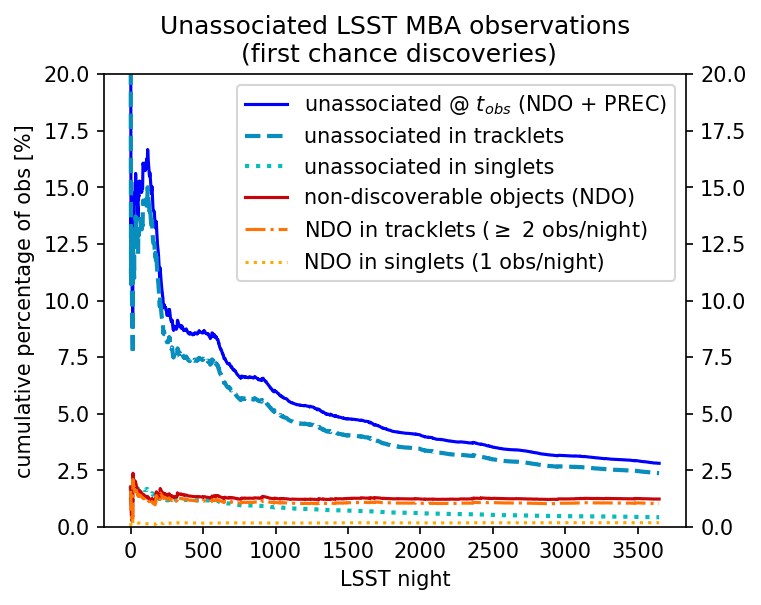
\includegraphics[width=0.70\linewidth]{figs/unasoc_frac_first_chance2.png}
%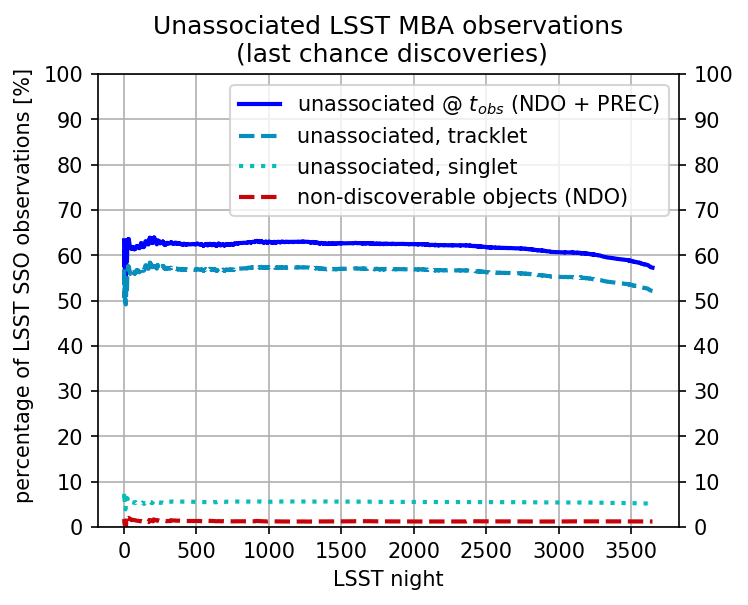
\includegraphics[width=0.50\linewidth]{figs/unasoc_frac_last_chance3.png}
\end{tabular}
\end{center}
\caption{Fraction of unassociated and non-discoverable object observations of MBAs assuming all asteroids have been discovered at the first opportunity.  \label{fig:ufc} }
%\caption{Left: Fraction of unassociated and non-discoverable object observations of MBAs assuming all asteroids have been discovered at the first opportunity. Right: All asteroids have been discovered at the last opportunity. \label{fig:ufc} }
\end{figure}
We distinguish between observations of 
\begin{itemize}
\item bright objects that are known today accounting for approximately 30\% of \gls{LSST} \gls{SSO} observations,
\item observations of non-discoverable objects (NDOs), SSOs that cannot be grouped into "three nighters", 
\item and unassociated observations, i.e. observations of NDOs and objects that have not been discovered at the \gls{epoch} of observation.
\end{itemize}
%
\begin{figure}[tb!]
\begin{center}
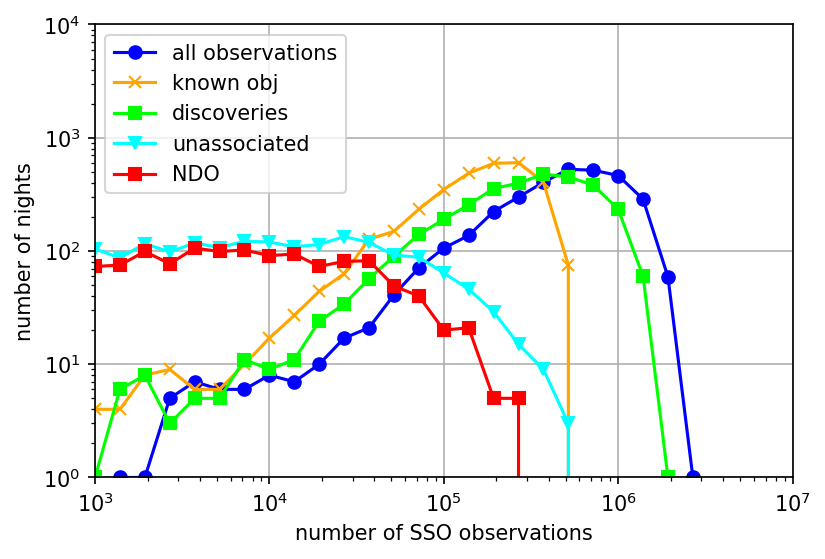
\includegraphics[width=0.7\linewidth]{figs/nights_vs_obs.png} 
\end{center}
\caption{Frequency of nights with a given number of observations.\label{fig:obs_stats}}
       % Give a unique label
\end{figure}
If asteroids are discovered early in the survey, e.g. with the first discovery opportunity, practically all \gls{LSST} observations of asteroids can be associated with SSOs after ten years of operations. Figure \ref{fig:ufc} as well as the data displayed in Table \ref{tab:mbaobs} underline this fact. 
However, the fraction of unassociated observations remains non-negligible throughout the survey.  
Figure \ref{fig:ufc} shows that that fraction is around 15\% at the beginning of the \gls{LSST} survey compared to merely 2.5\% near the end. This is not surprising as the fraction of discovered to undiscovered objects increases over time.
%The longer Solar System Processing is delayed, however, the more significant the fraction of observations that will remain unassociated. 
%In this context unassociated means that observations cannot not be attributed to a known or newly discovered object at the time of observation potentially triggering LSST alerts. 
Precovery algorithms can reduce the number of unassociated observations by roughly 50\%, but only a posteriori. 
At the time of observation, unassociated observations may still trigger unwanted \gls{LSST} alerts. 
Figure \ref{fig:obs_stats} suggests that most nights tend to have a relatively low number of unassociated observations, typically between 1k-10k (Table \ref{tab:obs_stats}). Similarly, one can expect between 100 and 10k observations from non-discoverable objects per night. Only a hand-full of nights may prove to be ``noisier".
Figure \ref{fig:ndo_h} shows the absolute magnitude distribution of detected, discovered and non-discovered objects for the MBA population model A.
One can see that the \gls{LSST} MBA survey is bound to discover practically all objects down to absolute magnitude $H=19.5$mag. The 50\% completeness mark is $H=21.5$mag.
Absolute magnitudes for non-discoverable objects range from H=19mag to H=25mag.
The on-sky distribution of observations of non-discoverable objects is shown in Figure \ref{fig:ndo_obs_sky}. The distribution broadly resembles the one in Figure \ref{fig:ndo_obs_sky}. Over ten years of operations, one would expect fewer than 4000 observations per square degree from non-discoverable MBAs near the ecliptic with an all-sky median value of 76 per night (\ref{tab:obs_stats}).   
%
\begin{table}[tb!]
\begin{center}
\begin{tabular}{lccccc}
\multicolumn{5}{c}{LSST Observations of MBAs}\\
\hline\hline
per night & all obs. & discoveries & known obj. & \gls{UNO} & \gls{NDO} \\\hline
median  & 528,022 &312,077  &177,172 &626 &72 \\
mean & 621,084 & 402,334 & 193,570 & 17,490 & 7,688 \\
std. dev. & 511,835 & 363,013& 145,676 &47,643 & 24,491\\
maximum & 2,976,668 & 2,134,030 & 683,392 & 656,687 & 356,857\\
\hline\hline\\
\end{tabular}
\end{center}
\caption{Nightly statistics for all \gls{LSST} MBA observations, currently known object observations, unassociated observations and observations of
non-discoverable objects.}
\label{tab:obs_stats}
\end{table}
%

\begin{figure}[tb!]
\begin{center}
\begin{tabular}{cc}
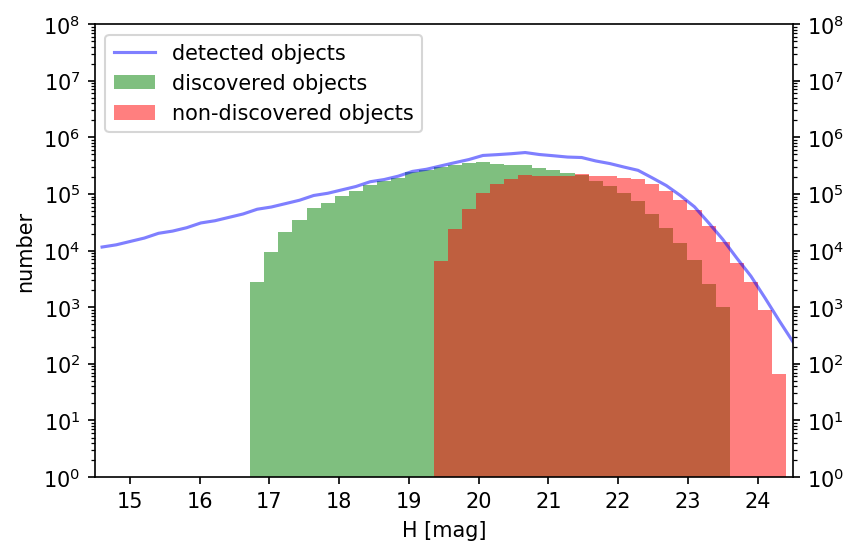
\includegraphics[width=0.70\linewidth]{figs/detection_discovered2.png}
\end{tabular}
\end{center}
\caption{Number of detected, discovered and non-discovered MBAs as a function of their absolute magnitude H. }
\label{fig:ndo_h}       % Give a unique label
\end{figure}

\begin{table}[tb!]
\begin{center}
\begin{tabular}{lcccccc}
\multicolumn{7}{c}{LSST Observations of MBAs}\\
\hline
Discovery at & Total & $H<14.5$mag & \gls{UNO} TR & \gls{UNO} SNGL & \gls{NDO} TR & \gls{NDO} SNGL \\
\hline
first chance & 2.27e+09 & 7.06e+08 & 5.39e+07 & 9.86e+06 & 2.37e+07 & 4.36e+06 \\
percentage   & 100\%  & 31.2\% & 2.4\% & 0.4\% & 1.1\% & 0.2\% \\\hline
%last chance & - & - & 1.18e+09 & 1.17e+08 & - & -  \\
%percentage   & - & - & 52.1\% & 5.2\% & -  & -\\
\hline
\end{tabular}
\end{center}
\caption{Main Belt Asteroid (MBA) observations at the end of the \gls{LSST} survey. Observations of bright, already known objects are in the column $H<14.5$mag.
Unassociated observations (\gls{UNO}) can partly be linked to discovered objects via \gls{precovery}. NDOs are observations of non-discoverable objects. The number of observations that are part of tracklets (TR) is contrasted with single observations per night (SNGL). Dashes indicate the first and last chance observations are the same.\label{tab:mbaobs}}
\end{table}

\begin{figure}[tb!]
\begin{center}
\begin{tabular}{cc}
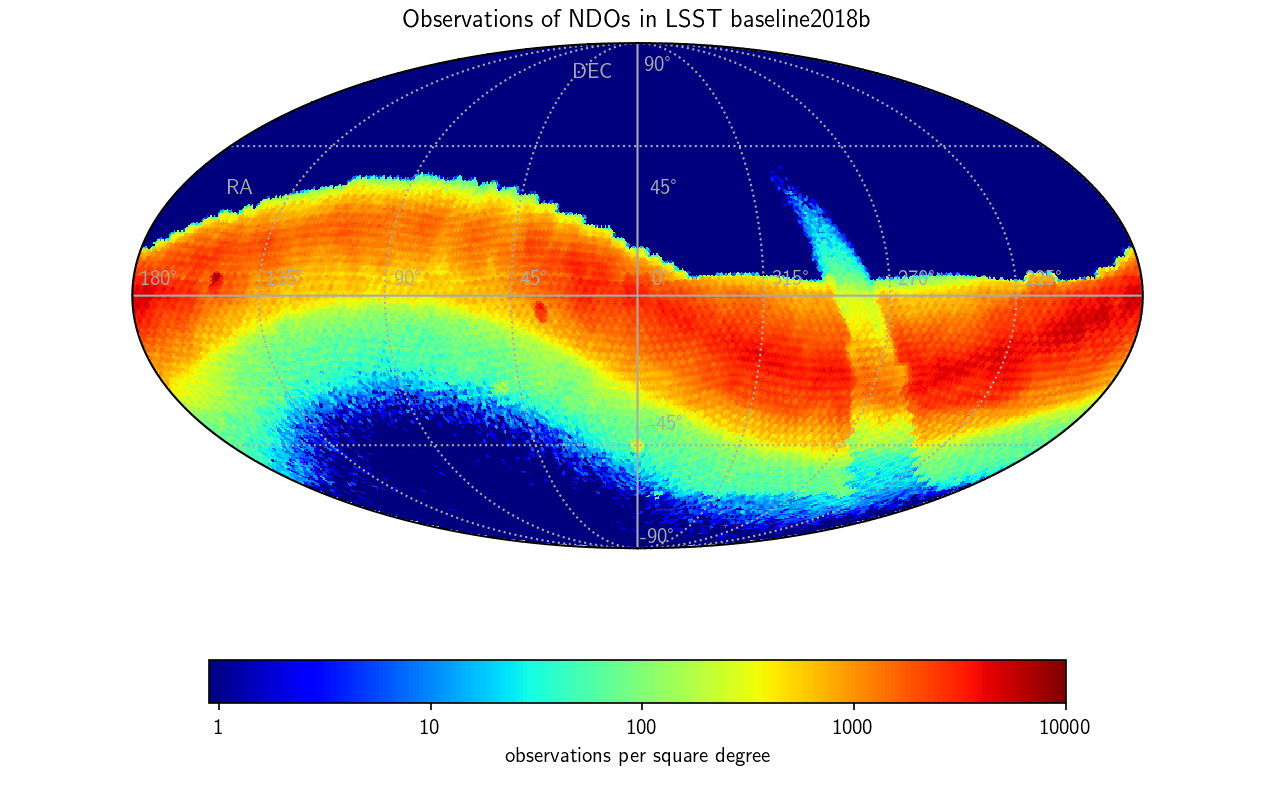
\includegraphics[width=0.80\linewidth]{figs/mba_obs_hp_ndo.png} &
\end{tabular}
\end{center}
\caption{On-sky distribution of observations per square degree of non-discoverable objects (NDOs).  }
\label{fig:ndo_obs_sky}       % Give a unique label
\end{figure}


\section{Expected \gls{MPC} Data Rates}\label{sec:data}
Based on observation statistics presented in the previous section we can estimate nightly data rates for submitting \gls{SSO} observations to the \gls{MPC}. The new Astrometry Data Exchange Standard (\gls{ADES}) submission format\footnote{\url{https://www.minorplanetcenter.net/iau/info/ADES.html}} that will be adopted by the time \gls{LSST} goes on line permits a more detailed description of optical observations of SSOs. Observation covariance information can be provided, for instance. As such, each observation should have an equivalent size of roughly 500bytes when submitted to the \gls{MPC}. Figure \ref{fig:data} shows the corresponding, expected nightly data volumes. Submissions will typically be on the order of several hundred MBs per night. \gls{GB} sized submissions are fairly rare occurring on roughly 50 nights during the ten years of \gls{LSST} operations. Given the fairly steep size-frequency distribution in population model A that has been used in this assessment, observations of new discoveries will dominate \gls{MPC} submissions despite the fact that known objects are brighter and tend to have more observations per object. Table \ref{tab:data_stats} contains the corresponding statistics. It is currently not planned to submit all observations to the \gls{MPC}. Only observations
that can be linked to known objects and those that can be confidently attributed new discoveries are to be delivered. 


\begin{figure}[tb!]
\begin{center}
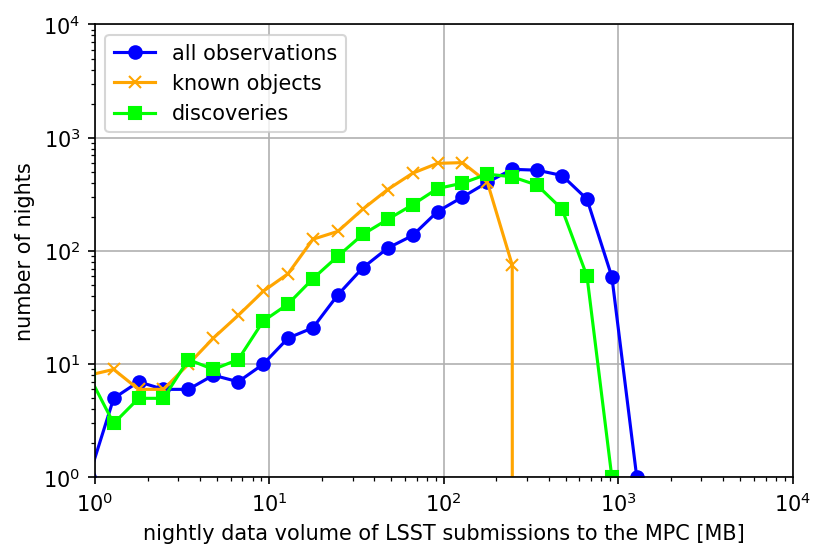
\includegraphics[width=0.70\linewidth]{figs/data2.png}
\end{center}
\caption{Predicted nightly data volumes for submissions of \gls{LSST} observations to the Minor Planet \gls{Center}.}
\label{fig:data}       % Give a unique label
\end{figure}
\clearpage

\begin{table}[tb!]
\begin{center}
\begin{tabular}{lccc}
\multicolumn{4}{c}{LSST data volumes for \gls{MPC} submission in \gls{ADES} format [MB]}\\
\hline\hline
per night & all obs. & discoveries & known obj. \\\hline
median  & 252 &149  &84  \\
mean & 296 & 192 & 92   \\
std. dev. & 244 & 173& 69 \\
maximum & 1,419 & 1,018 & 326 \\
\hline\hline\\
\end{tabular}
\end{center}
\caption{Nightly data volumes for the submission of \gls{LSST} MBA observations, discoveries and currently known object observations to the Minor Planet \gls{Center} in MegaBytes.}
\label{tab:data_stats}
\end{table}

\section{Other Solar System \gls{Object} populations}\label{sec:other}
Similar to the inner Solar System, size frequency distributions for SSOs in the outer solar system are not well understood. 
For Trojans and Trans-Neptunian Objects (TNOs) only cumulative completeness estimates are available this point. Those are presented in Figure \ref{fig:allcum}.
Until updated figures become available we suggest to use the previous predictions of 40k Trojan and 280k \gls{TNO} discoveries from \citet{jones2015asteroid}.
Interstellar objects and comets have not yet been investigated in detail.

\begin{figure}[tb!]
\begin{center}
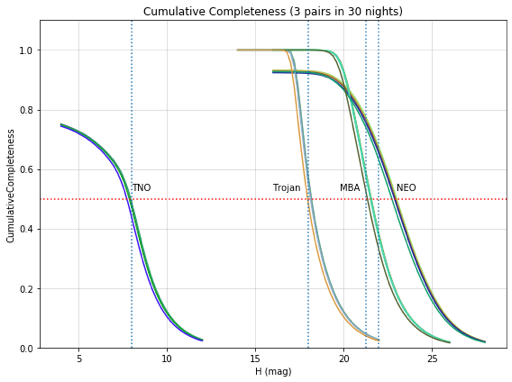
\includegraphics[width=0.60\linewidth]{figs/allcum.png}
\end{center}
\caption{Cumulative completeness for various solar system populations with the Feature Based Scheduler 1.2 baseline.
The two lines show results with visit pairs in the same filter vs. pairs in different filters (TNOs with C colors)}
\label{fig:allcum}       % Give a unique label
\end{figure}


\section{Conclusions} \label{sec:conclusions}

LSST is going to be the largest contributor of Solar System object observations and discoveries to be processed by the \gls{IAU} Minor Planet \gls{Center}.
The study at hand shows that
\begin{itemize}
\item \gls{LSST} is bound to discover between 49k-93k near-Earth asteroids (NEOs) depending on the actual size-frequency distribution.
\item Observations and discoveries of Main belt asteroids (MBAs) are bound to dominate \gls{LSST} \gls{SSO} data submitted to the \gls{IAU} Minor Planet \gls{Center}.
\item The number of MBAs discovered over 10 years of \gls{LSST} likely ranges between 4.8M and 5.4M and is unlikely to be higher than 220M. 
\item The majority of discoveries are going to be made within the first 2 to 3 years of the \gls{LSST} survey.
\item The number of MBA discoveries per night can be up to 100 000 with an average of 2000 for the most likely size-frequency distribution (population model A). Even in the unlikely case of a \gls{TNO}-like size-frequency distribution in the Main Belt we expect no more than 3 million discoveries per night on a handful of nights during the survey.
\item The vast majority of asteroids observed with \gls{LSST} have two and more observations per night.  
\item The "three nighter" paradigm for detecting SSOs leads to a non-negligible fraction of unattributable observations, since not all observations that can be connected into tracklets occur on three separate nights. 
\item After ten years of \gls{LSST} operations observations of non-discoverable objects are likely to be on the order of several thousands per square degree concentrated in a band around the ecliptic. This excludes TNOs that are too slow to be identified as moving objects. 
\item Nightly data volumes delivered to the Minor Planet \gls{Center} are generally on the order of several hundred MBs and only rarely exceed a \gls{GB}.
\end{itemize}


\appendix
% Include all the relevant bib files.
% https://lsst-texmf.lsst.io/lsstdoc.html#bibliographies
%\section{References}
\label{sec:bib}
\bibliography{lsst,lsst-dm,refs_ads,refs,books}

%Make sure lsst-texmf/bin/generateAcronyms.py is in your path
%\section{Acronyms used in this document}\label{sec:acronyms}
%\addtocounter{table}{-1}
\begin{longtable}{|l|p{0.8\textwidth}|}\hline
\textbf{Acronym} & \textbf{Description}  \\\hline

B & Byte (8 bit) \\\hline
DM & Data Management \\\hline
DMTN & DM Technical Note \\\hline
GB & Gigabyte \\\hline
IAU & International Astronomical Union \\\hline
JPL & Jet Propulsion Laboratory (DE ephemerides) \\\hline
LSST & Large Synoptic Survey Telescope \\\hline
MB & MegaByte \\\hline
NASA & National Aeronautics and Space Administration \\\hline
NEO & Near-Earth Object \\\hline
Pan-STARRS & Panoramic Survey Telescope and Rapid Response System \\\hline
XMM & X-ray Multi-mirror Mission (ESA; officially known as XMM-Newton) \\\hline
\end{longtable}

%Unccomment these if you want old style acronyms
\label{sec:acronyms}
\printglossaries

\end{document}
